\documentclass[twoside]{book}

% Packages required by doxygen
\usepackage{fixltx2e}
\usepackage{calc}
\usepackage{doxygen}
\usepackage{graphicx}
\usepackage[utf8]{inputenc}
\usepackage{makeidx}
\usepackage{multicol}
\usepackage{multirow}
\PassOptionsToPackage{warn}{textcomp}
\usepackage{textcomp}
\usepackage[nointegrals]{wasysym}
\usepackage[table]{xcolor}

% Font selection
\usepackage[T1]{fontenc}
\usepackage{mathptmx}
\usepackage[scaled=.90]{helvet}
\usepackage{courier}
\usepackage{amssymb}
\usepackage{sectsty}
\renewcommand{\familydefault}{\sfdefault}
\allsectionsfont{%
  \fontseries{bc}\selectfont%
  \color{darkgray}%
}
\renewcommand{\DoxyLabelFont}{%
  \fontseries{bc}\selectfont%
  \color{darkgray}%
}
\newcommand{\+}{\discretionary{\mbox{\scriptsize$\hookleftarrow$}}{}{}}

% Page & text layout
\usepackage{geometry}
\geometry{%
  a4paper,%
  top=2.5cm,%
  bottom=2.5cm,%
  left=2.5cm,%
  right=2.5cm%
}
\tolerance=750
\hfuzz=15pt
\hbadness=750
\setlength{\emergencystretch}{15pt}
\setlength{\parindent}{0cm}
\setlength{\parskip}{0.2cm}
\makeatletter
\renewcommand{\paragraph}{%
  \@startsection{paragraph}{4}{0ex}{-1.0ex}{1.0ex}{%
    \normalfont\normalsize\bfseries\SS@parafont%
  }%
}
\renewcommand{\subparagraph}{%
  \@startsection{subparagraph}{5}{0ex}{-1.0ex}{1.0ex}{%
    \normalfont\normalsize\bfseries\SS@subparafont%
  }%
}
\makeatother

% Headers & footers
\usepackage{fancyhdr}
\pagestyle{fancyplain}
\fancyhead[LE]{\fancyplain{}{\bfseries\thepage}}
\fancyhead[CE]{\fancyplain{}{}}
\fancyhead[RE]{\fancyplain{}{\bfseries\leftmark}}
\fancyhead[LO]{\fancyplain{}{\bfseries\rightmark}}
\fancyhead[CO]{\fancyplain{}{}}
\fancyhead[RO]{\fancyplain{}{\bfseries\thepage}}
\fancyfoot[LE]{\fancyplain{}{}}
\fancyfoot[CE]{\fancyplain{}{}}
\fancyfoot[RE]{\fancyplain{}{\bfseries\scriptsize Generated on Tue Oct 7 2014 17\+:36\+:04 for Min\+G++ I\+D\+E -\/ 2014 by Doxygen }}
\fancyfoot[LO]{\fancyplain{}{\bfseries\scriptsize Generated on Tue Oct 7 2014 17\+:36\+:04 for Min\+G++ I\+D\+E -\/ 2014 by Doxygen }}
\fancyfoot[CO]{\fancyplain{}{}}
\fancyfoot[RO]{\fancyplain{}{}}
\renewcommand{\footrulewidth}{0.4pt}
\renewcommand{\chaptermark}[1]{%
  \markboth{#1}{}%
}
\renewcommand{\sectionmark}[1]{%
  \markright{\thesection\ #1}%
}

% Indices & bibliography
\usepackage{natbib}
\usepackage[titles]{tocloft}
\setcounter{tocdepth}{3}
\setcounter{secnumdepth}{5}
\makeindex

% Hyperlinks (required, but should be loaded last)
\usepackage{ifpdf}
\ifpdf
  \usepackage[pdftex,pagebackref=true]{hyperref}
\else
  \usepackage[ps2pdf,pagebackref=true]{hyperref}
\fi
\hypersetup{%
  colorlinks=true,%
  linkcolor=blue,%
  citecolor=blue,%
  unicode%
}

% Custom commands
\newcommand{\clearemptydoublepage}{%
  \newpage{\pagestyle{empty}\cleardoublepage}%
}


%===== C O N T E N T S =====

\begin{document}

% Titlepage & ToC
\hypersetup{pageanchor=false,
             bookmarks=true,
             bookmarksnumbered=true,
             pdfencoding=unicode
            }
\pagenumbering{roman}
\begin{titlepage}
\vspace*{7cm}
\begin{center}%
{\Large Min\+G++ I\+D\+E -\/ 2014 \\[1ex]\large 0.\+1 (Pre-\/\+Alpha) }\\
\vspace*{1cm}
{\large Generated by Doxygen 1.8.8}\\
\vspace*{0.5cm}
{\small Tue Oct 7 2014 17:36:04}\\
\end{center}
\end{titlepage}
\clearemptydoublepage
\tableofcontents
\clearemptydoublepage
\pagenumbering{arabic}
\hypersetup{pageanchor=true}

%--- Begin generated contents ---
\chapter{Hierarchical Index}
\section{Class Hierarchy}
This inheritance list is sorted roughly, but not completely, alphabetically\+:\begin{DoxyCompactList}
\item \contentsline{section}{Common\+Info}{\pageref{struct_common_info}}{}
\item \contentsline{section}{Language\+Info}{\pageref{struct_language_info}}{}
\item \contentsline{section}{Style\+Info}{\pageref{struct_style_info}}{}
\item wx\+Dialog\begin{DoxyCompactList}
\item \contentsline{section}{Edit\+Properties}{\pageref{class_edit_properties}}{}
\item \contentsline{section}{New\+Dialog}{\pageref{class_new_dialog}}{}
\item \contentsline{section}{New\+File}{\pageref{class_new_file}}{}
\end{DoxyCompactList}
\item wx\+Frame\begin{DoxyCompactList}
\item \contentsline{section}{My\+Frame}{\pageref{class_my_frame}}{}
\end{DoxyCompactList}
\item wx\+Styled\+Text\+Ctrl\begin{DoxyCompactList}
\item \contentsline{section}{Edit}{\pageref{class_edit}}{}
\end{DoxyCompactList}
\end{DoxyCompactList}

\chapter{Class Index}
\section{Class List}
Here are the classes, structs, unions and interfaces with brief descriptions\+:\begin{DoxyCompactList}
\item\contentsline{section}{\hyperlink{struct_common_info}{Common\+Info} }{\pageref{struct_common_info}}{}
\item\contentsline{section}{\hyperlink{class_edit}{Edit} \\*\hyperlink{class_edit}{Edit} }{\pageref{class_edit}}{}
\item\contentsline{section}{\hyperlink{class_edit_properties}{Edit\+Properties} \\*\hyperlink{class_edit_properties}{Edit\+Properties} }{\pageref{class_edit_properties}}{}
\item\contentsline{section}{\hyperlink{struct_language_info}{Language\+Info} }{\pageref{struct_language_info}}{}
\item\contentsline{section}{\hyperlink{class_my_frame}{My\+Frame} }{\pageref{class_my_frame}}{}
\item\contentsline{section}{\hyperlink{class_new_dialog}{New\+Dialog} }{\pageref{class_new_dialog}}{}
\item\contentsline{section}{\hyperlink{class_new_file}{New\+File} }{\pageref{class_new_file}}{}
\item\contentsline{section}{\hyperlink{struct_style_info}{Style\+Info} }{\pageref{struct_style_info}}{}
\end{DoxyCompactList}

\chapter{Class Documentation}
\hypertarget{struct_common_info}{\section{Common\+Info Struct Reference}
\label{struct_common_info}\index{Common\+Info@{Common\+Info}}
}
\subsection*{Public Attributes}
\begin{DoxyCompactItemize}
\item 
\hypertarget{struct_common_info_a99a413cd9da7d4e1049eb0bce98065d2}{bool {\bfseries syntax\+Enable}}\label{struct_common_info_a99a413cd9da7d4e1049eb0bce98065d2}

\item 
\hypertarget{struct_common_info_a1bcd80ac2c2134e3fe43f7d82ac1f850}{bool {\bfseries fold\+Enable}}\label{struct_common_info_a1bcd80ac2c2134e3fe43f7d82ac1f850}

\item 
\hypertarget{struct_common_info_a7104659d4f2ced727fe5bd5a3adca7c0}{bool {\bfseries indent\+Enable}}\label{struct_common_info_a7104659d4f2ced727fe5bd5a3adca7c0}

\item 
\hypertarget{struct_common_info_a8922f6c9eb080084a5370e0ea7b5b775}{bool {\bfseries read\+Only\+Initial}}\label{struct_common_info_a8922f6c9eb080084a5370e0ea7b5b775}

\item 
\hypertarget{struct_common_info_a26e98e62bfc97ec7f394841c1253c109}{bool {\bfseries over\+Type\+Initial}}\label{struct_common_info_a26e98e62bfc97ec7f394841c1253c109}

\item 
\hypertarget{struct_common_info_aff7a584d1c2884bfd082fd9ea0269ba7}{bool {\bfseries wrap\+Mode\+Initial}}\label{struct_common_info_aff7a584d1c2884bfd082fd9ea0269ba7}

\item 
\hypertarget{struct_common_info_abb34cd44d96ba84f2019e46a8d651c6d}{bool {\bfseries display\+E\+O\+L\+Enable}}\label{struct_common_info_abb34cd44d96ba84f2019e46a8d651c6d}

\item 
\hypertarget{struct_common_info_a248215d39f176a1d1d8a6e1fe213d960}{bool {\bfseries indent\+Guide\+Enable}}\label{struct_common_info_a248215d39f176a1d1d8a6e1fe213d960}

\item 
\hypertarget{struct_common_info_ad17f055b76e26532fe03af219ee14c13}{bool {\bfseries line\+Number\+Enable}}\label{struct_common_info_ad17f055b76e26532fe03af219ee14c13}

\item 
\hypertarget{struct_common_info_acb671c443595c7065a6a8fe5a22dfcf4}{bool {\bfseries long\+Line\+On\+Enable}}\label{struct_common_info_acb671c443595c7065a6a8fe5a22dfcf4}

\item 
\hypertarget{struct_common_info_a5478324f28d021402e4c5ca4859217f2}{bool {\bfseries white\+Space\+Enable}}\label{struct_common_info_a5478324f28d021402e4c5ca4859217f2}

\end{DoxyCompactItemize}


The documentation for this struct was generated from the following file\+:\begin{DoxyCompactItemize}
\item 
prefs.\+h\end{DoxyCompactItemize}

\hypertarget{class_edit}{\section{Edit Class Reference}
\label{class_edit}\index{Edit@{Edit}}
}


\hyperlink{class_edit}{Edit}.  




{\ttfamily \#include $<$edit.\+h$>$}

Inheritance diagram for Edit\+:\begin{figure}[H]
\begin{center}
\leavevmode
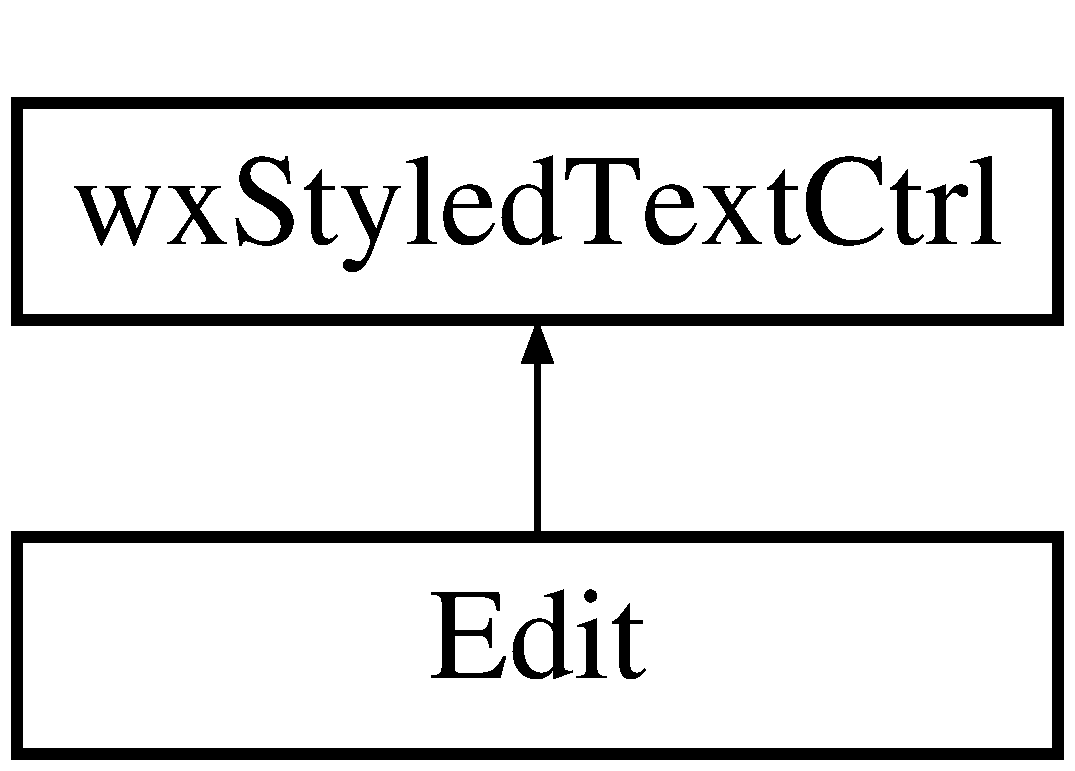
\includegraphics[height=2.000000cm]{class_edit}
\end{center}
\end{figure}
\subsection*{Public Member Functions}
\begin{DoxyCompactItemize}
\item 
\hypertarget{class_edit_af83e3ad6078bdd00f0e5d8a6bce44e04}{\hyperlink{class_edit_af83e3ad6078bdd00f0e5d8a6bce44e04}{Edit} (wx\+Window $\ast$parent, wx\+Window\+I\+D id=wx\+I\+D\+\_\+\+A\+N\+Y, const wx\+Point \&pos=wx\+Default\+Position, const wx\+Size \&size=wx\+Default\+Size, long style=wx\+S\+U\+N\+K\+E\+N\+\_\+\+B\+O\+R\+D\+E\+R$\vert$wx\+V\+S\+C\+R\+O\+L\+L)}\label{class_edit_af83e3ad6078bdd00f0e5d8a6bce44e04}

\begin{DoxyCompactList}\small\item\em constructor \end{DoxyCompactList}\item 
\hypertarget{class_edit_a999416ba7b28de1d62c69aab8697606a}{\hyperlink{class_edit_a999416ba7b28de1d62c69aab8697606a}{$\sim$\+Edit} ()}\label{class_edit_a999416ba7b28de1d62c69aab8697606a}

\begin{DoxyCompactList}\small\item\em destructor \end{DoxyCompactList}\item 
\hypertarget{class_edit_a6b58abb4839a26010df91fabfdd34e76}{void {\bfseries On\+Size} (wx\+Size\+Event \&event)}\label{class_edit_a6b58abb4839a26010df91fabfdd34e76}

\item 
\hypertarget{class_edit_a54cd90b0450b676cbe8c3fee8ca56a2a}{void {\bfseries On\+Edit\+Redo} (wx\+Command\+Event \&event)}\label{class_edit_a54cd90b0450b676cbe8c3fee8ca56a2a}

\item 
\hypertarget{class_edit_ab5f41eb566e0c5ad039fce444bf0b739}{void {\bfseries On\+Edit\+Undo} (wx\+Command\+Event \&event)}\label{class_edit_ab5f41eb566e0c5ad039fce444bf0b739}

\item 
\hypertarget{class_edit_ac57c3eabcfe4b9b4b43c31e81c959e8c}{void {\bfseries On\+Edit\+Clear} (wx\+Command\+Event \&event)}\label{class_edit_ac57c3eabcfe4b9b4b43c31e81c959e8c}

\item 
\hypertarget{class_edit_a27aba2b8a97702245e8c8623ad67fe21}{void {\bfseries On\+Edit\+Cut} (wx\+Command\+Event \&event)}\label{class_edit_a27aba2b8a97702245e8c8623ad67fe21}

\item 
\hypertarget{class_edit_a2478644d3faf1cc46b30519fb47abe35}{void {\bfseries On\+Edit\+Copy} (wx\+Command\+Event \&event)}\label{class_edit_a2478644d3faf1cc46b30519fb47abe35}

\item 
\hypertarget{class_edit_a88d1917bd250026e892b641aa3978241}{void {\bfseries On\+Edit\+Paste} (wx\+Command\+Event \&event)}\label{class_edit_a88d1917bd250026e892b641aa3978241}

\item 
\hypertarget{class_edit_a9342c879dadcc5cc13a8d5a3a33d4487}{void {\bfseries On\+Find} (wx\+Command\+Event \&event)}\label{class_edit_a9342c879dadcc5cc13a8d5a3a33d4487}

\item 
\hypertarget{class_edit_a428a613ac9e6081dc27b1660e28b0cf3}{void {\bfseries On\+Find\+Next} (wx\+Command\+Event \&event)}\label{class_edit_a428a613ac9e6081dc27b1660e28b0cf3}

\item 
\hypertarget{class_edit_ad4eb02f4e36b02050b9220604e95d8cb}{void {\bfseries On\+Replace} (wx\+Command\+Event \&event)}\label{class_edit_ad4eb02f4e36b02050b9220604e95d8cb}

\item 
\hypertarget{class_edit_a014b36331a97d3957c2e4b24cb5c6c46}{void {\bfseries On\+Replace\+Next} (wx\+Command\+Event \&event)}\label{class_edit_a014b36331a97d3957c2e4b24cb5c6c46}

\item 
\hypertarget{class_edit_a9dd0ae369b07ad6be4686c95ce013761}{void {\bfseries On\+Brace\+Match} (wx\+Command\+Event \&event)}\label{class_edit_a9dd0ae369b07ad6be4686c95ce013761}

\item 
\hypertarget{class_edit_a0ab101c0f8abfddd483ef135984020b1}{void {\bfseries On\+Goto} (wx\+Command\+Event \&event)}\label{class_edit_a0ab101c0f8abfddd483ef135984020b1}

\item 
\hypertarget{class_edit_aa006c200e66edd5ae1e4c6af280da613}{void {\bfseries On\+Edit\+Indent\+Inc} (wx\+Command\+Event \&event)}\label{class_edit_aa006c200e66edd5ae1e4c6af280da613}

\item 
\hypertarget{class_edit_a4a1956c8b612a86a76d9c7449bef73d2}{void {\bfseries On\+Edit\+Indent\+Red} (wx\+Command\+Event \&event)}\label{class_edit_a4a1956c8b612a86a76d9c7449bef73d2}

\item 
\hypertarget{class_edit_a2f326c611b3f72c06c818be0b5d03632}{void {\bfseries On\+Edit\+Select\+All} (wx\+Command\+Event \&event)}\label{class_edit_a2f326c611b3f72c06c818be0b5d03632}

\item 
\hypertarget{class_edit_a80ea201355875d8e3ff9d81c020b3ca9}{void {\bfseries On\+Edit\+Select\+Line} (wx\+Command\+Event \&event)}\label{class_edit_a80ea201355875d8e3ff9d81c020b3ca9}

\item 
\hypertarget{class_edit_abd88efa68e008e6cf0a4e8ddd9368fe0}{void \hyperlink{class_edit_abd88efa68e008e6cf0a4e8ddd9368fe0}{On\+Hilight\+Lang} (wx\+Command\+Event \&event)}\label{class_edit_abd88efa68e008e6cf0a4e8ddd9368fe0}

\begin{DoxyCompactList}\small\item\em view \end{DoxyCompactList}\item 
\hypertarget{class_edit_a88467f6e3d41e6c00311a43c9f8c2a2f}{void {\bfseries On\+Display\+E\+O\+L} (wx\+Command\+Event \&event)}\label{class_edit_a88467f6e3d41e6c00311a43c9f8c2a2f}

\item 
\hypertarget{class_edit_a51bbb55708c41ded2dfa5a4d87d07978}{void {\bfseries On\+Indent\+Guide} (wx\+Command\+Event \&event)}\label{class_edit_a51bbb55708c41ded2dfa5a4d87d07978}

\item 
\hypertarget{class_edit_a8262aca5bb842786dc1dc1fc2360659e}{void {\bfseries On\+Line\+Number} (wx\+Command\+Event \&event)}\label{class_edit_a8262aca5bb842786dc1dc1fc2360659e}

\item 
\hypertarget{class_edit_a67c8747c802b8ddde2f3a1e58f457093}{void {\bfseries On\+Long\+Line\+On} (wx\+Command\+Event \&event)}\label{class_edit_a67c8747c802b8ddde2f3a1e58f457093}

\item 
\hypertarget{class_edit_a3303108fe64cfd7c5a62355fff38d727}{void {\bfseries On\+White\+Space} (wx\+Command\+Event \&event)}\label{class_edit_a3303108fe64cfd7c5a62355fff38d727}

\item 
\hypertarget{class_edit_af168157256af6f29c4c549d24707b1f1}{void {\bfseries On\+Fold\+Toggle} (wx\+Command\+Event \&event)}\label{class_edit_af168157256af6f29c4c549d24707b1f1}

\item 
\hypertarget{class_edit_a7ba02b7307434853f23c787f858dd10e}{void {\bfseries On\+Set\+Over\+Type} (wx\+Command\+Event \&event)}\label{class_edit_a7ba02b7307434853f23c787f858dd10e}

\item 
\hypertarget{class_edit_a28f90e2baa3b28cb5cb72578f41c1b6a}{void {\bfseries On\+Set\+Read\+Only} (wx\+Command\+Event \&event)}\label{class_edit_a28f90e2baa3b28cb5cb72578f41c1b6a}

\item 
\hypertarget{class_edit_aa10e8f9dc7a7dcec051832e2bce186fa}{void {\bfseries On\+Wrapmode\+On} (wx\+Command\+Event \&event)}\label{class_edit_aa10e8f9dc7a7dcec051832e2bce186fa}

\item 
\hypertarget{class_edit_a94585b38355ccbadc7550e17f7ccb320}{void {\bfseries On\+Use\+Charset} (wx\+Command\+Event \&event)}\label{class_edit_a94585b38355ccbadc7550e17f7ccb320}

\item 
\hypertarget{class_edit_aba8807e4d99524b9ebec4dff2501720c}{void {\bfseries On\+Annotation\+Add} (wx\+Command\+Event \&event)}\label{class_edit_aba8807e4d99524b9ebec4dff2501720c}

\item 
\hypertarget{class_edit_a990bc053deb4490d21aee2c978d0c5b1}{void {\bfseries On\+Annotation\+Remove} (wx\+Command\+Event \&event)}\label{class_edit_a990bc053deb4490d21aee2c978d0c5b1}

\item 
\hypertarget{class_edit_ac4b693934cbc7e0478bbef89e28a1a2f}{void {\bfseries On\+Annotation\+Clear} (wx\+Command\+Event \&event)}\label{class_edit_ac4b693934cbc7e0478bbef89e28a1a2f}

\item 
\hypertarget{class_edit_a81e4aba09a6269ed023d59d6f441c079}{void {\bfseries On\+Annotation\+Style} (wx\+Command\+Event \&event)}\label{class_edit_a81e4aba09a6269ed023d59d6f441c079}

\item 
\hypertarget{class_edit_a35f2c182c8161d70df526d7ac672598d}{void \hyperlink{class_edit_a35f2c182c8161d70df526d7ac672598d}{On\+Change\+Case} (wx\+Command\+Event \&event)}\label{class_edit_a35f2c182c8161d70df526d7ac672598d}

\begin{DoxyCompactList}\small\item\em extra \end{DoxyCompactList}\item 
\hypertarget{class_edit_aa9765073b671289574f6e69b377e3b5f}{void {\bfseries On\+Convert\+E\+O\+L} (wx\+Command\+Event \&event)}\label{class_edit_aa9765073b671289574f6e69b377e3b5f}

\item 
\hypertarget{class_edit_ab02764c433061f10bfc4b66c0662c014}{void \hyperlink{class_edit_ab02764c433061f10bfc4b66c0662c014}{On\+Margin\+Click} (wx\+Styled\+Text\+Event \&event)}\label{class_edit_ab02764c433061f10bfc4b66c0662c014}

\begin{DoxyCompactList}\small\item\em misc \end{DoxyCompactList}\item 
\hypertarget{class_edit_acfd8c8e7e830f6417f7b2a60c13a44c9}{void {\bfseries On\+Char\+Added} (wx\+Styled\+Text\+Event \&event)}\label{class_edit_acfd8c8e7e830f6417f7b2a60c13a44c9}

\item 
\hypertarget{class_edit_aa81c0098ff533b01c17f1d49d63a3122}{void {\bfseries On\+Key} (wx\+Styled\+Text\+Event \&event)}\label{class_edit_aa81c0098ff533b01c17f1d49d63a3122}

\item 
\hypertarget{class_edit_a84aa2d6a1789d6eb223cf410c2cd75ee}{void {\bfseries Add\+Breakpoint} (wx\+String path, int add\+Line)}\label{class_edit_a84aa2d6a1789d6eb223cf410c2cd75ee}

\item 
\hypertarget{class_edit_aae5ca34dcf1a83e592d346ec18387d4e}{void {\bfseries Remove\+Breakpoint} (wx\+String path, int remove\+Line)}\label{class_edit_aae5ca34dcf1a83e592d346ec18387d4e}

\item 
\hypertarget{class_edit_ad3fe918901eba29c8626ea340b8ecb20}{wx\+String \hyperlink{class_edit_ad3fe918901eba29c8626ea340b8ecb20}{Determine\+Prefs} (const wx\+String \&filename)}\label{class_edit_ad3fe918901eba29c8626ea340b8ecb20}

\begin{DoxyCompactList}\small\item\em language/lexer \end{DoxyCompactList}\item 
\hypertarget{class_edit_ace7f1699b31d98f6a65b6c8a5d7a1e7a}{bool {\bfseries Initialize\+Prefs} (const wx\+String \&filename)}\label{class_edit_ace7f1699b31d98f6a65b6c8a5d7a1e7a}

\item 
\hypertarget{class_edit_a4aabee0c58f1a7d5c06a6d84f53e9dd3}{bool {\bfseries User\+Settings} (const wx\+String \&filename)}\label{class_edit_a4aabee0c58f1a7d5c06a6d84f53e9dd3}

\item 
\hypertarget{class_edit_af4247fd6b08b2c537de6578a21ffe831}{\hyperlink{struct_language_info}{Language\+Info} const $\ast$ {\bfseries Get\+Language\+Info} ()}\label{class_edit_af4247fd6b08b2c537de6578a21ffe831}

\item 
\hypertarget{class_edit_a451e2cce5f283792f69af5b3909d0331}{bool \hyperlink{class_edit_a451e2cce5f283792f69af5b3909d0331}{Load\+File} ()}\label{class_edit_a451e2cce5f283792f69af5b3909d0331}

\begin{DoxyCompactList}\small\item\em load/save file \end{DoxyCompactList}\item 
\hypertarget{class_edit_ac84a22d579dcdb7775babd33cc044d47}{bool {\bfseries Load\+File} (const wx\+String \&filename)}\label{class_edit_ac84a22d579dcdb7775babd33cc044d47}

\item 
\hypertarget{class_edit_a5e3471365aed52be41de12daef848b5e}{bool {\bfseries Save\+File} ()}\label{class_edit_a5e3471365aed52be41de12daef848b5e}

\item 
\hypertarget{class_edit_a1620e4a99e0b65ef666f268d80db4898}{bool {\bfseries Save\+File} (const wx\+String \&filename)}\label{class_edit_a1620e4a99e0b65ef666f268d80db4898}

\item 
\hypertarget{class_edit_a93d3a59290d5a495aa9cddeaa7e9a96b}{bool {\bfseries Modified} ()}\label{class_edit_a93d3a59290d5a495aa9cddeaa7e9a96b}

\item 
\hypertarget{class_edit_a6f19e24819e7896ec01865db806ba349}{wx\+String {\bfseries Get\+Filename} ()}\label{class_edit_a6f19e24819e7896ec01865db806ba349}

\item 
\hypertarget{class_edit_ad86746317aa9a859da185d24df285710}{void {\bfseries Set\+Filename} (const wx\+String \&filename)}\label{class_edit_ad86746317aa9a859da185d24df285710}

\end{DoxyCompactItemize}
\subsection*{Public Attributes}
\begin{DoxyCompactItemize}
\item 
\hypertarget{class_edit_a6043a48f640f5ef2c1782282056c1dc9}{vector$<$ int $>$ {\bfseries breakpointsvec}}\label{class_edit_a6043a48f640f5ef2c1782282056c1dc9}

\item 
\hypertarget{class_edit_a6584a73601846b51c879a6d326fbb5f9}{bool {\bfseries breakpoint\+\_\+flag}}\label{class_edit_a6584a73601846b51c879a6d326fbb5f9}

\item 
\hypertarget{class_edit_ae685b10b41d57c5e65cc7c77f42d432d}{int {\bfseries breakline}}\label{class_edit_ae685b10b41d57c5e65cc7c77f42d432d}

\item 
\hypertarget{class_edit_a7a6f572c876e229c95d3294a62035958}{int {\bfseries deleteline}}\label{class_edit_a7a6f572c876e229c95d3294a62035958}

\end{DoxyCompactItemize}
\subsection*{Friends}
\begin{DoxyCompactItemize}
\item 
\hypertarget{class_edit_a500387361234a2fd8343f4673951f68d}{class {\bfseries Edit\+Properties}}\label{class_edit_a500387361234a2fd8343f4673951f68d}

\item 
\hypertarget{class_edit_abe05a77802c8bdef1ff7bdc9171d4391}{class {\bfseries Edit\+Print}}\label{class_edit_abe05a77802c8bdef1ff7bdc9171d4391}

\end{DoxyCompactItemize}


\subsection{Detailed Description}
\hyperlink{class_edit}{Edit}. 

The documentation for this class was generated from the following files\+:\begin{DoxyCompactItemize}
\item 
edit.\+h\item 
edit.\+cpp\end{DoxyCompactItemize}

\hypertarget{class_edit_properties}{\section{Edit\+Properties Class Reference}
\label{class_edit_properties}\index{Edit\+Properties@{Edit\+Properties}}
}


\hyperlink{class_edit_properties}{Edit\+Properties}.  




{\ttfamily \#include $<$edit.\+h$>$}

Inheritance diagram for Edit\+Properties\+:\begin{figure}[H]
\begin{center}
\leavevmode
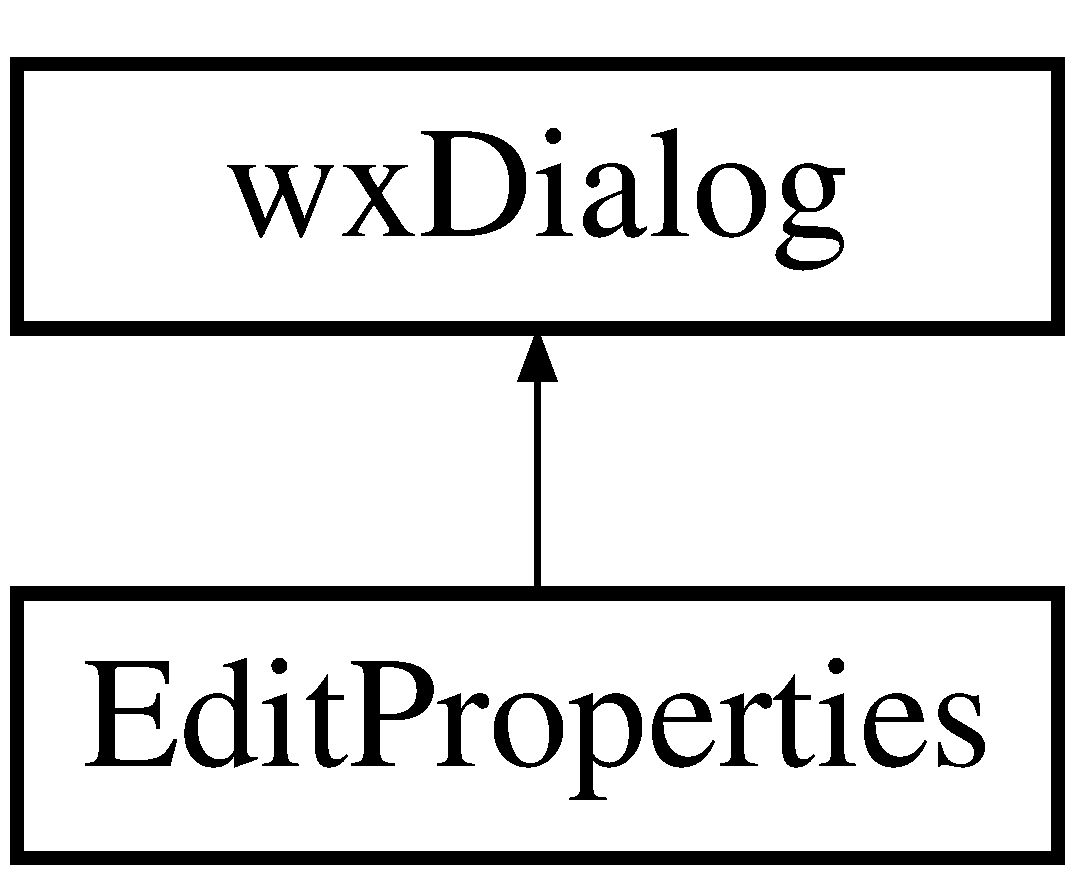
\includegraphics[height=2.000000cm]{class_edit_properties}
\end{center}
\end{figure}
\subsection*{Public Member Functions}
\begin{DoxyCompactItemize}
\item 
\hypertarget{class_edit_properties_ad3cf2454738d0e76238dfbcb0fb3b7ff}{\hyperlink{class_edit_properties_ad3cf2454738d0e76238dfbcb0fb3b7ff}{Edit\+Properties} (\hyperlink{class_edit}{Edit} $\ast$edit, long style=0)}\label{class_edit_properties_ad3cf2454738d0e76238dfbcb0fb3b7ff}

\begin{DoxyCompactList}\small\item\em constructor \end{DoxyCompactList}\end{DoxyCompactItemize}


\subsection{Detailed Description}
\hyperlink{class_edit_properties}{Edit\+Properties}. 

The documentation for this class was generated from the following files\+:\begin{DoxyCompactItemize}
\item 
edit.\+h\item 
edit.\+cpp\end{DoxyCompactItemize}

\hypertarget{struct_language_info}{\section{Language\+Info Struct Reference}
\label{struct_language_info}\index{Language\+Info@{Language\+Info}}
}
\subsection*{Public Attributes}
\begin{DoxyCompactItemize}
\item 
\hypertarget{struct_language_info_a0bc62ed7957ef0fa887b0b82bfd2dc9c}{const char $\ast$ {\bfseries name}}\label{struct_language_info_a0bc62ed7957ef0fa887b0b82bfd2dc9c}

\item 
\hypertarget{struct_language_info_aed06ca491cbda9c51355e5c960fc3cba}{const char $\ast$ {\bfseries filepattern}}\label{struct_language_info_aed06ca491cbda9c51355e5c960fc3cba}

\item 
\hypertarget{struct_language_info_a3a632e8ed1bc3173c9be39834e60eee3}{int {\bfseries lexer}}\label{struct_language_info_a3a632e8ed1bc3173c9be39834e60eee3}

\item 
\hypertarget{struct_language_info_aa365f6f9328f2ba5dd8a54aa1b6ee401}{\begin{tabbing}
xx\=xx\=xx\=xx\=xx\=xx\=xx\=xx\=xx\=\kill
struct \{\\
\>int {\bfseries type}\\
\>const char $\ast$ {\bfseries words}\\
\} {\bfseries styles} \mbox{[}STYLE\_TYPES\_COUNT\mbox{]}}\label{struct_language_info_aa365f6f9328f2ba5dd8a54aa1b6ee401}
\\

\end{tabbing}\item 
\hypertarget{struct_language_info_af24520623253cd01e5aac96cd1c625a9}{int {\bfseries folds}}\label{struct_language_info_af24520623253cd01e5aac96cd1c625a9}

\end{DoxyCompactItemize}


The documentation for this struct was generated from the following file\+:\begin{DoxyCompactItemize}
\item 
prefs.\+h\end{DoxyCompactItemize}

\hypertarget{class_my_frame}{\section{My\+Frame Class Reference}
\label{class_my_frame}\index{My\+Frame@{My\+Frame}}
}
Inheritance diagram for My\+Frame\+:\begin{figure}[H]
\begin{center}
\leavevmode
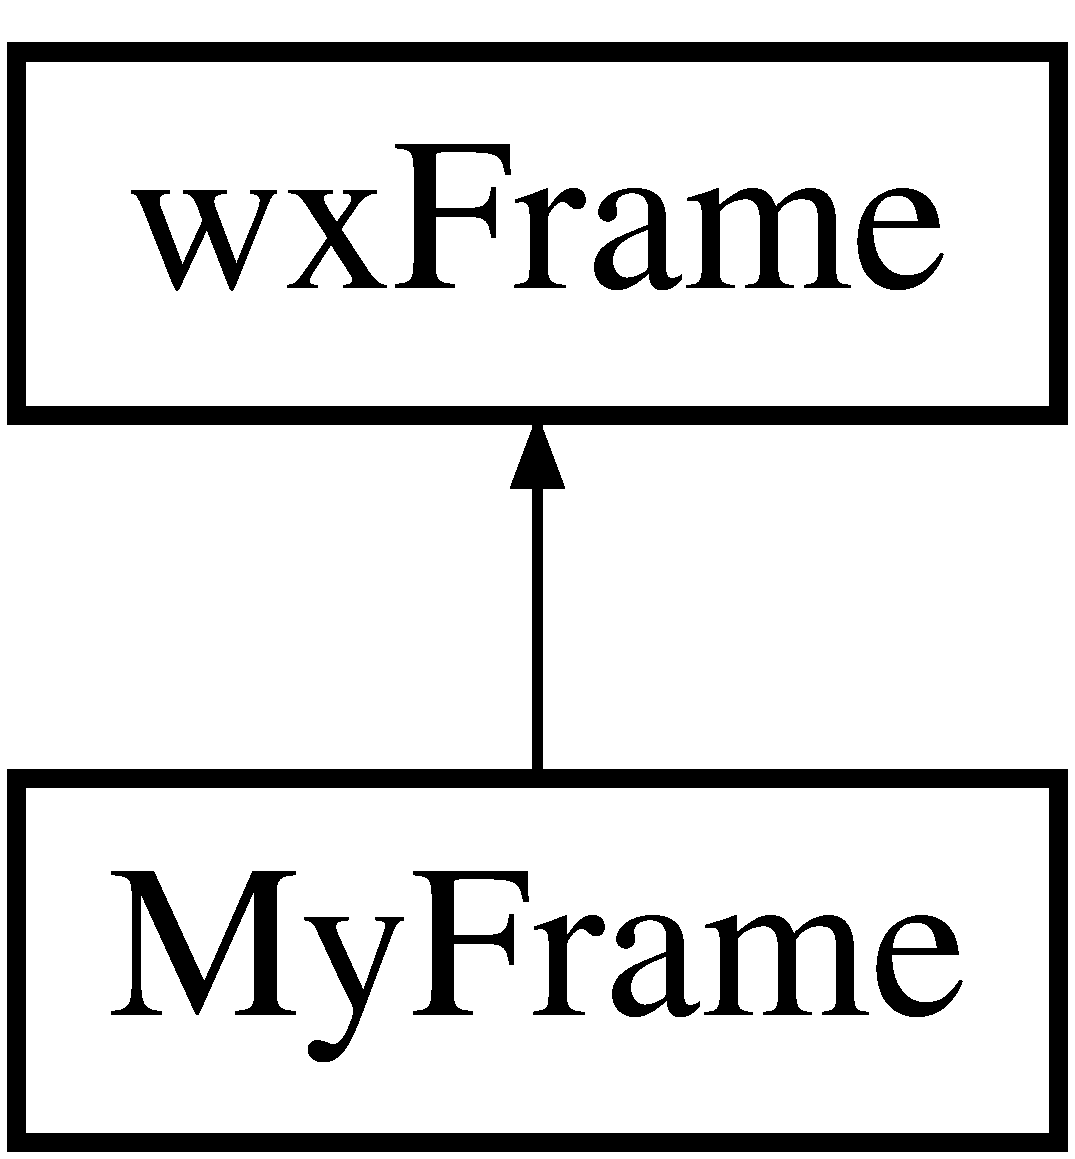
\includegraphics[height=2.000000cm]{class_my_frame}
\end{center}
\end{figure}
\subsection*{Public Types}
\begin{DoxyCompactItemize}
\item 
\hypertarget{class_my_frame_aa3aa7ed18d345c10376374ce7e5ec703}{typedef wx\+Tree\+Item\+Id(wx\+Tree\+Ctrl\+::$\ast$ {\bfseries Tree\+Func0\+\_\+t} )() const }\label{class_my_frame_aa3aa7ed18d345c10376374ce7e5ec703}

\item 
\hypertarget{class_my_frame_a49114c539b71c6f4c18d7a4858b5b171}{typedef wx\+Tree\+Item\+Id(wx\+Tree\+Ctrl\+::$\ast$ {\bfseries Tree\+Func1\+\_\+t} )(const wx\+Tree\+Item\+Id \&) const }\label{class_my_frame_a49114c539b71c6f4c18d7a4858b5b171}

\end{DoxyCompactItemize}
\subsection*{Public Member Functions}
\begin{DoxyCompactItemize}
\item 
\hypertarget{class_my_frame_adb0ef0657ae6da07cfc9b5cb97bf830e}{void {\bfseries Get\+Items\+Recursively} (const wx\+Tree\+Item\+Id \&id\+Parent, wx\+Tree\+Item\+Id\+Value cookie=0)}\label{class_my_frame_adb0ef0657ae6da07cfc9b5cb97bf830e}

\item 
\hypertarget{class_my_frame_ae61088e3c39f47de93cfee6a431ff8c7}{void {\bfseries Add\+Test\+Items\+To\+Tree} (size\+\_\+t num\+Children, size\+\_\+t depth)}\label{class_my_frame_ae61088e3c39f47de93cfee6a431ff8c7}

\item 
\hypertarget{class_my_frame_ae914b83cd080c0fbf45998c14cf66b40}{void {\bfseries On\+Save\+Solution} (wx\+Tree\+Item\+Id solution)}\label{class_my_frame_ae914b83cd080c0fbf45998c14cf66b40}

\item 
\hypertarget{class_my_frame_a9562ec6151b8c4286f389dd482bb1e57}{void {\bfseries File\+Open} (wx\+String fname)}\label{class_my_frame_a9562ec6151b8c4286f389dd482bb1e57}

\item 
\hypertarget{class_my_frame_a2e7388f928078b7451d2a8456beb8fd1}{void {\bfseries On\+Notebook\+Page\+Closed} (wx\+Aui\+Notebook\+Event \&event)}\label{class_my_frame_a2e7388f928078b7451d2a8456beb8fd1}

\item 
\hypertarget{class_my_frame_a0f2ce68a3e90bd2f69b4180530c10744}{void {\bfseries On\+File\+New} (wx\+Command\+Event \&event)}\label{class_my_frame_a0f2ce68a3e90bd2f69b4180530c10744}

\item 
\hypertarget{class_my_frame_a5293d0ca07360b7cdc8cdde42634b6de}{void {\bfseries On\+Item\+R\+Click} (wx\+Tree\+Event \&event)}\label{class_my_frame_a5293d0ca07360b7cdc8cdde42634b6de}

\item 
\hypertarget{class_my_frame_a1cbcc149bf0319a52311e5fbf66ae4d4}{void {\bfseries On\+New\+File} (wx\+Command\+Event \&event)}\label{class_my_frame_a1cbcc149bf0319a52311e5fbf66ae4d4}

\item 
\hypertarget{class_my_frame_a4c5effeba4519bd2d8b2a19000beb5b2}{void {\bfseries On\+File\+Project} (wx\+Command\+Event \&event)}\label{class_my_frame_a4c5effeba4519bd2d8b2a19000beb5b2}

\item 
\hypertarget{class_my_frame_ad74164812c96ccffaab0a838ad3ec5c4}{void {\bfseries On\+Load\+Project} (wx\+Command\+Event \&event)}\label{class_my_frame_ad74164812c96ccffaab0a838ad3ec5c4}

\item 
\hypertarget{class_my_frame_aa86080f2ffa1c07a135d694ba769d5fe}{void {\bfseries On\+Save\+Project} (wx\+Command\+Event \&event)}\label{class_my_frame_aa86080f2ffa1c07a135d694ba769d5fe}

\item 
\hypertarget{class_my_frame_a6b3f9709ddfc01c14d06f7f630d5f7d8}{void {\bfseries On\+File\+New\+Frame} (wx\+Command\+Event \&event)}\label{class_my_frame_a6b3f9709ddfc01c14d06f7f630d5f7d8}

\item 
\hypertarget{class_my_frame_a9b559c7ef01b41e31e88e05bf410a39b}{void {\bfseries On\+File\+Open} (wx\+Command\+Event \&event)}\label{class_my_frame_a9b559c7ef01b41e31e88e05bf410a39b}

\item 
\hypertarget{class_my_frame_a2cda7ffa7a914f8a6e9722cfc61ec68b}{void {\bfseries On\+File\+Open\+Frame} (wx\+Command\+Event \&event)}\label{class_my_frame_a2cda7ffa7a914f8a6e9722cfc61ec68b}

\item 
\hypertarget{class_my_frame_a755476d85a15af2da071de070812d953}{void {\bfseries On\+File\+Save} (wx\+Command\+Event \&event)}\label{class_my_frame_a755476d85a15af2da071de070812d953}

\item 
\hypertarget{class_my_frame_a4e693828efb571fb2992d0afbf851963}{void {\bfseries On\+File\+Save\+As} (wx\+Command\+Event \&event)}\label{class_my_frame_a4e693828efb571fb2992d0afbf851963}

\item 
\hypertarget{class_my_frame_aacab35fe30d1d45944307c71a4179ea1}{void {\bfseries On\+File\+Close} (wx\+Command\+Event \&event)}\label{class_my_frame_aacab35fe30d1d45944307c71a4179ea1}

\item 
\hypertarget{class_my_frame_ab72daefc5a74695f02427ae126df7261}{void {\bfseries On\+Exit} (wx\+Command\+Event \&event)}\label{class_my_frame_ab72daefc5a74695f02427ae126df7261}

\item 
\hypertarget{class_my_frame_ab470cba0c5d8d46980c602589d556ee5}{void {\bfseries On\+About} (wx\+Command\+Event \&event)}\label{class_my_frame_ab470cba0c5d8d46980c602589d556ee5}

\item 
\hypertarget{class_my_frame_a81f3ca63a2546ed79772b12fa1ed4860}{void {\bfseries On\+Compile} (wx\+Command\+Event \&event)}\label{class_my_frame_a81f3ca63a2546ed79772b12fa1ed4860}

\item 
\hypertarget{class_my_frame_a107bbf19b177e4f2d2759f8450dbd4fe}{void {\bfseries On\+Build} (wx\+Command\+Event \&event)}\label{class_my_frame_a107bbf19b177e4f2d2759f8450dbd4fe}

\item 
\hypertarget{class_my_frame_aff26e8d2566067e0a24a2516cf6ce4d6}{void {\bfseries On\+Re\+Build} (wx\+Command\+Event \&event)}\label{class_my_frame_aff26e8d2566067e0a24a2516cf6ce4d6}

\item 
\hypertarget{class_my_frame_ad61fe77b26b2c496f6d0298d9983ce78}{void {\bfseries On\+Clean} (wx\+Command\+Event \&event)}\label{class_my_frame_ad61fe77b26b2c496f6d0298d9983ce78}

\item 
\hypertarget{class_my_frame_a1f3d07e0f3b8faced4f900c91e4125ca}{void {\bfseries On\+Start} (wx\+Command\+Event \&event)}\label{class_my_frame_a1f3d07e0f3b8faced4f900c91e4125ca}

\item 
\hypertarget{class_my_frame_a4c6b9b384c8aa4bba4003ac4df76d43a}{void {\bfseries On\+Debug} (wx\+Command\+Event \&W\+X\+U\+N\+U\+S\+E\+D(event))}\label{class_my_frame_a4c6b9b384c8aa4bba4003ac4df76d43a}

\item 
\hypertarget{class_my_frame_aca8e8d9ade335e41689ae7ccbbc8675a}{void {\bfseries On\+Close} (wx\+Close\+Event \&event)}\label{class_my_frame_aca8e8d9ade335e41689ae7ccbbc8675a}

\item 
\hypertarget{class_my_frame_a4bfc00e8a9e246cc4adf7f1d7e2e780f}{void {\bfseries On\+Timer} (wx\+Timer\+Event \&event)}\label{class_my_frame_a4bfc00e8a9e246cc4adf7f1d7e2e780f}

\item 
\hypertarget{class_my_frame_a718e57f55665880c50a717212b88932f}{void \hyperlink{class_my_frame_a718e57f55665880c50a717212b88932f}{On\+Properties} (wx\+Command\+Event \&event)}\label{class_my_frame_a718e57f55665880c50a717212b88932f}

\begin{DoxyCompactList}\small\item\em properties \end{DoxyCompactList}\item 
\hypertarget{class_my_frame_aa7e1c75cc203a03ec1ff13d0a193da34}{void {\bfseries Start\+Page} (wx\+Command\+Event \&event)}\label{class_my_frame_aa7e1c75cc203a03ec1ff13d0a193da34}

\item 
\hypertarget{class_my_frame_a5ebc2b26f4d86a1d0c29166ce6ce0996}{void {\bfseries On\+Property\+Page} (wx\+Command\+Event \&event)}\label{class_my_frame_a5ebc2b26f4d86a1d0c29166ce6ce0996}

\item 
\hypertarget{class_my_frame_a9e6c4824efad3aa9f4c3a3025a616e2d}{void {\bfseries On\+Quit} (wx\+Command\+Event \&event)}\label{class_my_frame_a9e6c4824efad3aa9f4c3a3025a616e2d}

\item 
\hypertarget{class_my_frame_ab9201004e1b94d87e4915507da4628e4}{void {\bfseries On\+Print\+Setup} (wx\+Command\+Event \&event)}\label{class_my_frame_ab9201004e1b94d87e4915507da4628e4}

\item 
\hypertarget{class_my_frame_a30d3a65aad431cb6d359a21e6b01f59c}{void {\bfseries On\+Print\+Preview} (wx\+Command\+Event \&event)}\label{class_my_frame_a30d3a65aad431cb6d359a21e6b01f59c}

\item 
\hypertarget{class_my_frame_a9b8443902bcd3be93a9103ede4247473}{void {\bfseries On\+Print} (wx\+Command\+Event \&event)}\label{class_my_frame_a9b8443902bcd3be93a9103ede4247473}

\item 
\hypertarget{class_my_frame_af36bfa551701f6d4e013182ffad407e5}{void {\bfseries On\+Tree\+Menu} (wx\+Tree\+Event \&event)}\label{class_my_frame_af36bfa551701f6d4e013182ffad407e5}

\item 
\hypertarget{class_my_frame_afc88a438cc4c6f1dd00a10e1836cb2e2}{void {\bfseries On\+Create\+Notebook} (wx\+String File\+Name)}\label{class_my_frame_afc88a438cc4c6f1dd00a10e1836cb2e2}

\item 
\hypertarget{class_my_frame_ac8b68e5ef6840b76a581fd6609b52a40}{void {\bfseries On\+Rename} (wx\+Command\+Event \&event)}\label{class_my_frame_ac8b68e5ef6840b76a581fd6609b52a40}

\item 
\hypertarget{class_my_frame_afa839d6dfb12f69cd8d5089af39754a6}{void {\bfseries On\+Delete} (wx\+Command\+Event \&event)}\label{class_my_frame_afa839d6dfb12f69cd8d5089af39754a6}

\item 
\hypertarget{class_my_frame_a8dc1c452bab299dacc6ddaf52b581986}{void {\bfseries On\+Item\+Menu} (wx\+Tree\+Event \&event)}\label{class_my_frame_a8dc1c452bab299dacc6ddaf52b581986}

\item 
\hypertarget{class_my_frame_a50c118fb4a8bb39fbfbb9a0ce7a40911}{void {\bfseries Show\+Menu} (wx\+Tree\+Item\+Id id, const wx\+Point \&pt)}\label{class_my_frame_a50c118fb4a8bb39fbfbb9a0ce7a40911}

\item 
\hypertarget{class_my_frame_a96c8023f2ec54d32f5d71bcfad79efef}{void {\bfseries On\+Begin\+Drag} (wx\+Tree\+Event \&event)}\label{class_my_frame_a96c8023f2ec54d32f5d71bcfad79efef}

\item 
\hypertarget{class_my_frame_a01ba8137f74f641f5eb26c031b7630dc}{void {\bfseries On\+Begin\+R\+Drag} (wx\+Tree\+Event \&event)}\label{class_my_frame_a01ba8137f74f641f5eb26c031b7630dc}

\item 
\hypertarget{class_my_frame_a9ffe045750dcaa4e93f18e88ac5bbb00}{void {\bfseries On\+End\+Drag} (wx\+Tree\+Event \&event)}\label{class_my_frame_a9ffe045750dcaa4e93f18e88ac5bbb00}

\item 
\hypertarget{class_my_frame_a128a48a72829fe283bb29f4a7e752523}{void {\bfseries On\+Begin\+Label\+Edit} (wx\+Tree\+Event \&event)}\label{class_my_frame_a128a48a72829fe283bb29f4a7e752523}

\item 
\hypertarget{class_my_frame_a2b2d2a5dcafc8c14b0979d51921d289b}{void {\bfseries On\+End\+Label\+Edit} (wx\+Tree\+Event \&event)}\label{class_my_frame_a2b2d2a5dcafc8c14b0979d51921d289b}

\item 
\hypertarget{class_my_frame_aa0ec35bcf43a39a1aa9f7ffe1c6cded0}{void {\bfseries On\+Delete\+Item} (wx\+Tree\+Event \&event)}\label{class_my_frame_aa0ec35bcf43a39a1aa9f7ffe1c6cded0}

\item 
\hypertarget{class_my_frame_abadf78efb6e5da62082ad02916124727}{void {\bfseries On\+Context\+Menu} (wx\+Context\+Menu\+Event \&event)}\label{class_my_frame_abadf78efb6e5da62082ad02916124727}

\item 
\hypertarget{class_my_frame_a56a049d6c0f2065a0e00442e061a7480}{void {\bfseries On\+Get\+Info} (wx\+Tree\+Event \&event)}\label{class_my_frame_a56a049d6c0f2065a0e00442e061a7480}

\item 
\hypertarget{class_my_frame_a2463050226a19a5ac018ff2646e775d7}{void {\bfseries On\+Set\+Info} (wx\+Tree\+Event \&event)}\label{class_my_frame_a2463050226a19a5ac018ff2646e775d7}

\item 
\hypertarget{class_my_frame_a841f627cf18feb4f0cf0ed2f7a18e92f}{void {\bfseries On\+Item\+Expanded} (wx\+Tree\+Event \&event)}\label{class_my_frame_a841f627cf18feb4f0cf0ed2f7a18e92f}

\item 
\hypertarget{class_my_frame_a7792f94a81b3a2721ef6cfd324524163}{void {\bfseries On\+Item\+Expanding} (wx\+Tree\+Event \&event)}\label{class_my_frame_a7792f94a81b3a2721ef6cfd324524163}

\item 
\hypertarget{class_my_frame_aa9b2cd47741e163cb4552d3c62ce63e2}{void {\bfseries On\+Item\+Collapsed} (wx\+Tree\+Event \&event)}\label{class_my_frame_aa9b2cd47741e163cb4552d3c62ce63e2}

\item 
\hypertarget{class_my_frame_abd896103559532bed8617606b1447930}{void {\bfseries On\+Item\+Collapsing} (wx\+Tree\+Event \&event)}\label{class_my_frame_abd896103559532bed8617606b1447930}

\item 
\hypertarget{class_my_frame_a6ceb19e603278d7b199b314e7f02f688}{void {\bfseries On\+Sel\+Changed} (wx\+Tree\+Event \&event)}\label{class_my_frame_a6ceb19e603278d7b199b314e7f02f688}

\item 
\hypertarget{class_my_frame_a212cea1f4caf2a697b3d8cd1251e5f50}{void {\bfseries On\+Sel\+Changing} (wx\+Tree\+Event \&event)}\label{class_my_frame_a212cea1f4caf2a697b3d8cd1251e5f50}

\item 
\hypertarget{class_my_frame_aee792b87ae25ee2026f2a8244653c464}{void {\bfseries On\+Tree\+Key\+Down} (wx\+Tree\+Event \&event)}\label{class_my_frame_aee792b87ae25ee2026f2a8244653c464}

\item 
\hypertarget{class_my_frame_af3d1463d4a80d4ece133d1d38782fa31}{void {\bfseries Load\+Tree\+Node\+State} (wx\+Xml\+Node $\ast$node)}\label{class_my_frame_af3d1463d4a80d4ece133d1d38782fa31}

\item 
\hypertarget{class_my_frame_a3f8790bd2add4e8a7a3cbc40c3ce9f5c}{void {\bfseries Save\+Tree\+Node\+State} (wx\+Tree\+Item\+Id id, wx\+Xml\+Node $\ast$node)}\label{class_my_frame_a3f8790bd2add4e8a7a3cbc40c3ce9f5c}

\item 
\hypertarget{class_my_frame_a15e642068698359c0e78ce263169e661}{void {\bfseries On\+Item\+Activated} (wx\+Tree\+Event \&event)}\label{class_my_frame_a15e642068698359c0e78ce263169e661}

\item 
\hypertarget{class_my_frame_af96760e4df77d847717e6afdf9cfec3e}{void {\bfseries On\+Item\+State\+Click} (wx\+Tree\+Event \&event)}\label{class_my_frame_af96760e4df77d847717e6afdf9cfec3e}

\item 
\hypertarget{class_my_frame_a24f5ddc6515b02efd2cb7079f42988b0}{void {\bfseries On\+R\+Mouse\+Down} (wx\+Mouse\+Event \&event)}\label{class_my_frame_a24f5ddc6515b02efd2cb7079f42988b0}

\item 
\hypertarget{class_my_frame_a2333ce08a9debddbad12c2ecf7abd1ba}{void {\bfseries On\+R\+Mouse\+Up} (wx\+Mouse\+Event \&event)}\label{class_my_frame_a2333ce08a9debddbad12c2ecf7abd1ba}

\item 
\hypertarget{class_my_frame_a8c4128e1104471317fd37e3985d9063f}{void {\bfseries On\+R\+Mouse\+D\+Click} (wx\+Mouse\+Event \&event)}\label{class_my_frame_a8c4128e1104471317fd37e3985d9063f}

\item 
\hypertarget{class_my_frame_a4d3bd40c8abd4779d62e388688b4b49e}{void {\bfseries On\+Process\+Term} (wx\+Process\+Event \&event)}\label{class_my_frame_a4d3bd40c8abd4779d62e388688b4b49e}

\item 
\hypertarget{class_my_frame_a6a4652f2e55b5be34781be6f936ee69d}{void {\bfseries Show\+Output} (const wx\+String \&cmd, const wx\+Array\+String \&output, const wx\+String \&title)}\label{class_my_frame_a6a4652f2e55b5be34781be6f936ee69d}

\item 
\hypertarget{class_my_frame_a695b023f086392b01e9bc35278a173e4}{void \hyperlink{class_my_frame_a695b023f086392b01e9bc35278a173e4}{On\+Edit} (wx\+Command\+Event \&event)}\label{class_my_frame_a695b023f086392b01e9bc35278a173e4}

\begin{DoxyCompactList}\small\item\em edit events \end{DoxyCompactList}\item 
\hypertarget{class_my_frame_a489f24a7f22c96c0db2428c56cc8fd23}{void {\bfseries Do\+Show\+First\+Or\+Last} (Tree\+Func0\+\_\+t pfn, const wx\+String \&label)}\label{class_my_frame_a489f24a7f22c96c0db2428c56cc8fd23}

\item 
\hypertarget{class_my_frame_a3b99729ec888ea071d7e43c5bda4dfd6}{void {\bfseries Do\+Show\+Relative\+Item} (Tree\+Func1\+\_\+t pfn, const wx\+String \&label)}\label{class_my_frame_a3b99729ec888ea071d7e43c5bda4dfd6}

\item 
\hypertarget{class_my_frame_a0a0c96d1c2ed63e1ed5ec760c264abd6}{wx\+Rect {\bfseries Determine\+Print\+Size} ()}\label{class_my_frame_a0a0c96d1c2ed63e1ed5ec760c264abd6}

\item 
\hypertarget{class_my_frame_af383f88851a6e4e47917a2f10abd0be3}{void {\bfseries Add\+Items\+Recursively} (const wx\+Tree\+Item\+Id \&id\+Parent, size\+\_\+t n\+Children, size\+\_\+t depth, size\+\_\+t folder)}\label{class_my_frame_af383f88851a6e4e47917a2f10abd0be3}

\item 
\hypertarget{class_my_frame_a994da93a143e19df0856168d785a471d}{{\bfseries My\+Frame} (wx\+Frame $\ast$parent, const wx\+String \&cmd, wx\+Process $\ast$process)}\label{class_my_frame_a994da93a143e19df0856168d785a471d}

\item 
\hypertarget{class_my_frame_a4e732ef446e650ed89ed7eb370bbedb4}{{\bfseries D\+E\+C\+L\+A\+R\+E\+\_\+\+E\+V\+E\+N\+T\+\_\+\+T\+A\+B\+L\+E} ()}\label{class_my_frame_a4e732ef446e650ed89ed7eb370bbedb4}

\item 
\hypertarget{class_my_frame_aa72c1011d890ebb970c10981d640b856}{void {\bfseries Do\+Get\+From\+Stream} (wx\+Text\+Ctrl $\ast$text, wx\+Input\+Stream \&in)}\label{class_my_frame_aa72c1011d890ebb970c10981d640b856}

\item 
\hypertarget{class_my_frame_a8d7783da2d823e4148d0517b74f90bad}{void {\bfseries Disable\+Input} ()}\label{class_my_frame_a8d7783da2d823e4148d0517b74f90bad}

\item 
\hypertarget{class_my_frame_a0ace815e204e10eacf8d60523668c7f9}{void {\bfseries Disable\+Output} ()}\label{class_my_frame_a0ace815e204e10eacf8d60523668c7f9}

\end{DoxyCompactItemize}
\subsection*{Public Attributes}
\begin{DoxyCompactItemize}
\item 
\hypertarget{class_my_frame_ad86fcc0424a94fa3e946a26dd65120c6}{wx\+Panel $\ast$ {\bfseries panel\+\_\+2}}\label{class_my_frame_ad86fcc0424a94fa3e946a26dd65120c6}

\item 
\hypertarget{class_my_frame_aee44d7b68ae0506211a96698b8090a2d}{wx\+Timer $\ast$ {\bfseries timer}}\label{class_my_frame_aee44d7b68ae0506211a96698b8090a2d}

\item 
\hypertarget{class_my_frame_a0d6783226c3fde78a48ea01dc657d760}{wx\+Aui\+Tool\+Bar $\ast$ {\bfseries tb2}}\label{class_my_frame_a0d6783226c3fde78a48ea01dc657d760}

\item 
\hypertarget{class_my_frame_a527ae7f85a0c0ed6ffe98a4e0abdd78f}{wx\+Aui\+Tool\+Bar $\ast$ {\bfseries tb3}}\label{class_my_frame_a527ae7f85a0c0ed6ffe98a4e0abdd78f}

\item 
\hypertarget{class_my_frame_af281e70f7e7a2ddc0a54dcab7b15e4a7}{bool {\bfseries issolution}}\label{class_my_frame_af281e70f7e7a2ddc0a54dcab7b15e4a7}

\item 
\hypertarget{class_my_frame_a1972c377c2a1b5963b55b8112847fed9}{bool {\bfseries start}}\label{class_my_frame_a1972c377c2a1b5963b55b8112847fed9}

\item 
\hypertarget{class_my_frame_af4a59e5d8424cf2c0a13bd63fec00099}{bool {\bfseries \+\_\+\+Debug}}\label{class_my_frame_af4a59e5d8424cf2c0a13bd63fec00099}

\item 
\hypertarget{class_my_frame_a37b984dcae136fd0d01f32d4ccf8a0d9}{bool {\bfseries savedfile}}\label{class_my_frame_a37b984dcae136fd0d01f32d4ccf8a0d9}

\item 
\hypertarget{class_my_frame_ad7975569b51d316f1005ada5a1cedee1}{wx\+Xml\+Node $\ast$ {\bfseries srcnode}}\label{class_my_frame_ad7975569b51d316f1005ada5a1cedee1}

\item 
\hypertarget{class_my_frame_a53e580bd2e33d91ac1c6e56be2717c6a}{wx\+Xml\+Node $\ast$ {\bfseries headernode}}\label{class_my_frame_a53e580bd2e33d91ac1c6e56be2717c6a}

\item 
\hypertarget{class_my_frame_a55fdc62db9cfaed55c9318a49a7e6d00}{wx\+Xml\+Node $\ast$ {\bfseries cpp}}\label{class_my_frame_a55fdc62db9cfaed55c9318a49a7e6d00}

\item 
\hypertarget{class_my_frame_a29d0500f3ac56fefc8754eb0f9655493}{wx\+Xml\+Node $\ast$ {\bfseries header}}\label{class_my_frame_a29d0500f3ac56fefc8754eb0f9655493}

\item 
\hypertarget{class_my_frame_a8219bad5739991ed403ad91e8e39b6da}{vector$<$ string $>$ {\bfseries filessrc}}\label{class_my_frame_a8219bad5739991ed403ad91e8e39b6da}

\item 
\hypertarget{class_my_frame_abe51d41c3d84769d73b644614e8b6dda}{vector$<$ string $>$ {\bfseries filesh}}\label{class_my_frame_abe51d41c3d84769d73b644614e8b6dda}

\item 
\hypertarget{class_my_frame_aad2347baa5785992e29c71072f7a4830}{\hyperlink{class_edit}{Edit} $\ast$ {\bfseries m\+\_\+edit}}\label{class_my_frame_aad2347baa5785992e29c71072f7a4830}

\item 
\hypertarget{class_my_frame_a487ae8aac4b7d05d5c943c3c2786b3c6}{wx\+Timer {\bfseries m\+\_\+timer}}\label{class_my_frame_a487ae8aac4b7d05d5c943c3c2786b3c6}

\item 
\hypertarget{class_my_frame_a0dd1da5220fb2ccde7c6e899a9ac9dce}{vector$<$ string $>$ {\bfseries soultionfilevec}}\label{class_my_frame_a0dd1da5220fb2ccde7c6e899a9ac9dce}

\item 
\hypertarget{class_my_frame_a5fabef1e36aeeff63246329a6f3a28c1}{wx\+Array\+Tree\+Item\+Ids {\bfseries itemsolutionid}}\label{class_my_frame_a5fabef1e36aeeff63246329a6f3a28c1}

\item 
\hypertarget{class_my_frame_aab3a8a461611c91fd0c0659e7c0a3dcd}{wx\+String {\bfseries fname}}\label{class_my_frame_aab3a8a461611c91fd0c0659e7c0a3dcd}

\item 
\hypertarget{class_my_frame_a63a7fedb7d8996df5cd2454365feea03}{wx\+String {\bfseries modt}}\label{class_my_frame_a63a7fedb7d8996df5cd2454365feea03}

\item 
\hypertarget{class_my_frame_a1025191d15a9aff70df9e77a159f7329}{wx\+Aui\+Notebook $\ast$ {\bfseries ctrl}}\label{class_my_frame_a1025191d15a9aff70df9e77a159f7329}

\item 
\hypertarget{class_my_frame_a9337781ba1d71d42971e02caea6d98e7}{wx\+Aui\+Notebook $\ast$ {\bfseries ctrl\+\_\+tree}}\label{class_my_frame_a9337781ba1d71d42971e02caea6d98e7}

\item 
\hypertarget{class_my_frame_acc62ca6e2ad9dd4915fcbdc2872479f2}{\hyperlink{class_new_dialog}{New\+Dialog} $\ast$ {\bfseries frame\+\_\+1}}\label{class_my_frame_acc62ca6e2ad9dd4915fcbdc2872479f2}

\item 
\hypertarget{class_my_frame_a3473a01c8aa7ef8a6c232111671c42d4}{\hyperlink{class_new_file}{New\+File} $\ast$ {\bfseries frame\+\_\+2}}\label{class_my_frame_a3473a01c8aa7ef8a6c232111671c42d4}

\item 
\hypertarget{class_my_frame_afcc5a6bb81b4974c02d844b902e4e961}{wx\+String {\bfseries workspace\+\_\+path}}\label{class_my_frame_afcc5a6bb81b4974c02d844b902e4e961}

\item 
\hypertarget{class_my_frame_a70626835d6e63d476a1092f802bec224}{wx\+String {\bfseries exe\+\_\+path}}\label{class_my_frame_a70626835d6e63d476a1092f802bec224}

\item 
\hypertarget{class_my_frame_a77bb008026eabc81bd2dca226816f12f}{wx\+String {\bfseries projpath}}\label{class_my_frame_a77bb008026eabc81bd2dca226816f12f}

\item 
\hypertarget{class_my_frame_a29aabdbfb2e175821dd36d7ad1aedebf}{wx\+Tree\+Ctrl $\ast$ {\bfseries tree}}\label{class_my_frame_a29aabdbfb2e175821dd36d7ad1aedebf}

\item 
\hypertarget{class_my_frame_a8d22151fc0ec200de05f325d6807f253}{wx\+Text\+Ctrl $\ast$ {\bfseries text2}}\label{class_my_frame_a8d22151fc0ec200de05f325d6807f253}

\item 
\hypertarget{class_my_frame_a1262cd98206b608f85470317dd529089}{wx\+Text\+Ctrl $\ast$ {\bfseries text3}}\label{class_my_frame_a1262cd98206b608f85470317dd529089}

\item 
\hypertarget{class_my_frame_a40a0dfa821d2cda71044997836653c66}{wx\+Text\+Ctrl $\ast$ {\bfseries text4}}\label{class_my_frame_a40a0dfa821d2cda71044997836653c66}

\item 
\hypertarget{class_my_frame_a6b16b3eafea902ae147d51bb3e9a2fe2}{wx\+Tree\+Ctrl $\ast$ {\bfseries list\+\_\+ctrl\+\_\+1}}\label{class_my_frame_a6b16b3eafea902ae147d51bb3e9a2fe2}

\item 
\hypertarget{class_my_frame_a0be74aac3ab23d4d7d16399a4101d135}{wx\+Generic\+Dir\+Ctrl $\ast$ {\bfseries list\+\_\+ctrl\+\_\+dir}}\label{class_my_frame_a0be74aac3ab23d4d7d16399a4101d135}

\item 
\hypertarget{class_my_frame_ab6efa33bd1fba44bbc839095d18016a8}{wx\+Image\+List $\ast$ {\bfseries imglist}}\label{class_my_frame_ab6efa33bd1fba44bbc839095d18016a8}

\item 
\hypertarget{class_my_frame_a8410311ea7dbf67ec6ace07a1916de50}{wx\+Html\+Window $\ast$ {\bfseries m\+\_\+\+Html}}\label{class_my_frame_a8410311ea7dbf67ec6ace07a1916de50}

\item 
\hypertarget{class_my_frame_aed5d4ec683f13148ff048ecc81922164}{wx\+Tree\+Item\+Id {\bfseries hid}}\label{class_my_frame_aed5d4ec683f13148ff048ecc81922164}

\item 
\hypertarget{class_my_frame_a7a561e671356fadfa6d1cc7deed8d448}{wx\+Tree\+Item\+Id {\bfseries srcid}}\label{class_my_frame_a7a561e671356fadfa6d1cc7deed8d448}

\item 
\hypertarget{class_my_frame_a3a91d099ae0373183fa00af75954c21a}{wx\+Html\+Easy\+Printing $\ast$ {\bfseries m\+\_\+\+Prn}}\label{class_my_frame_a3a91d099ae0373183fa00af75954c21a}

\item 
\hypertarget{class_my_frame_aed2b61e6306bb58a4e5bafe4175a81ea}{wx\+String {\bfseries m\+\_\+\+Name}}\label{class_my_frame_aed2b61e6306bb58a4e5bafe4175a81ea}

\item 
\hypertarget{class_my_frame_a3cdc00e9285a2e4f201230441978a8e2}{wx\+Tree\+Item\+Id {\bfseries m\+\_\+last\+Item}}\label{class_my_frame_a3cdc00e9285a2e4f201230441978a8e2}

\item 
\hypertarget{class_my_frame_a876353dbea98a5ea900d3ed855ad5c95}{wx\+Tree\+Item\+Id {\bfseries m\+\_\+dragged\+Item}}\label{class_my_frame_a876353dbea98a5ea900d3ed855ad5c95}

\item 
\hypertarget{class_my_frame_a6949f1a968302805b6c9cdc0d218c1b6}{long {\bfseries m\+\_\+notebook\+\_\+style}}\label{class_my_frame_a6949f1a968302805b6c9cdc0d218c1b6}

\item 
\hypertarget{class_my_frame_a5cdffae4c76ceda0d1d20f695ec08949}{long {\bfseries m\+\_\+notebook\+\_\+theme}}\label{class_my_frame_a5cdffae4c76ceda0d1d20f695ec08949}

\item 
\hypertarget{class_my_frame_a5267b957150143deab057b6b35835f3f}{wx\+Tree\+Item\+Id {\bfseries root}}\label{class_my_frame_a5267b957150143deab057b6b35835f3f}

\item 
\hypertarget{class_my_frame_a1b4172d1e07e8aca474e67fa44135dc1}{wx\+Array\+Tree\+Item\+Ids {\bfseries items}}\label{class_my_frame_a1b4172d1e07e8aca474e67fa44135dc1}

\item 
\hypertarget{class_my_frame_a88b786d4e235fefcc99f4d8b56e90523}{wx\+Aui\+Manager {\bfseries m\+\_\+mgr}}\label{class_my_frame_a88b786d4e235fefcc99f4d8b56e90523}

\item 
\hypertarget{class_my_frame_a899fbf04e5df65ec7b6fc71269bcf25a}{wx\+Property\+Grid $\ast$ {\bfseries m\+\_\+pg}}\label{class_my_frame_a899fbf04e5df65ec7b6fc71269bcf25a}

\item 
\hypertarget{class_my_frame_ad8bfcbab09df7b551e165b2009cac72c}{wx\+Process $\ast$ {\bfseries process}}\label{class_my_frame_ad8bfcbab09df7b551e165b2009cac72c}

\item 
\hypertarget{class_my_frame_a2c7a30fdcc0cc8aa606a09fde9913e02}{wx\+Process $\ast$ {\bfseries m\+\_\+process}}\label{class_my_frame_a2c7a30fdcc0cc8aa606a09fde9913e02}

\item 
\hypertarget{class_my_frame_a3b1abe02282d861862cdbc92fff7c761}{wx\+List\+Ctrl $\ast$ {\bfseries m\+\_\+item\+\_\+list}}\label{class_my_frame_a3b1abe02282d861862cdbc92fff7c761}

\item 
\hypertarget{class_my_frame_a588c67348c4b1edbf3aa6247fe564e60}{wx\+Output\+Stream \& {\bfseries m\+\_\+out}}\label{class_my_frame_a588c67348c4b1edbf3aa6247fe564e60}

\item 
\hypertarget{class_my_frame_aa388fe2f05a0a09ef5100556f6647876}{wx\+Input\+Stream \& {\bfseries m\+\_\+in}}\label{class_my_frame_aa388fe2f05a0a09ef5100556f6647876}

\item 
\hypertarget{class_my_frame_a0067d5751514b7b848796ba374784633}{wx\+Input\+Stream \& {\bfseries m\+\_\+err}}\label{class_my_frame_a0067d5751514b7b848796ba374784633}

\item 
\hypertarget{class_my_frame_ac2240983e92a9e82a46eae87e341d333}{wx\+Text\+Ctrl $\ast$ {\bfseries m\+\_\+text\+Out}}\label{class_my_frame_ac2240983e92a9e82a46eae87e341d333}

\item 
\hypertarget{class_my_frame_aba7629d74fabbfc2ee42caab01242ac5}{wx\+Text\+Ctrl $\ast$ {\bfseries m\+\_\+text\+In}}\label{class_my_frame_aba7629d74fabbfc2ee42caab01242ac5}

\item 
\hypertarget{class_my_frame_a8bed6a6ae541fdfdf52fde0e8c21abb3}{wx\+Text\+Ctrl $\ast$ {\bfseries m\+\_\+text\+Err}}\label{class_my_frame_a8bed6a6ae541fdfdf52fde0e8c21abb3}

\item 
\hypertarget{class_my_frame_aa022cd1b61ebb9a6aefb431f00c08f3f}{wx\+String {\bfseries \+\_\+\+Debug\+Str}}\label{class_my_frame_aa022cd1b61ebb9a6aefb431f00c08f3f}

\item 
\hypertarget{class_my_frame_ab118c814a6c0821cee40672fc52f1e29}{wx\+String {\bfseries cmdebug}}\label{class_my_frame_ab118c814a6c0821cee40672fc52f1e29}

\end{DoxyCompactItemize}
\subsection*{Static Public Attributes}
\begin{DoxyCompactItemize}
\item 
\hypertarget{class_my_frame_a6db4ee6efadd827b26b2c2cef819ee8b}{static bool {\bfseries ms\+\_\+log\+Text}}\label{class_my_frame_a6db4ee6efadd827b26b2c2cef819ee8b}

\item 
\hypertarget{class_my_frame_a6f0f6aa2427dac4e05ab0999991e19fc}{static bool {\bfseries ms\+\_\+log\+Focus}}\label{class_my_frame_a6f0f6aa2427dac4e05ab0999991e19fc}

\end{DoxyCompactItemize}
\subsection*{Protected Member Functions}
\begin{DoxyCompactItemize}
\item 
\hypertarget{class_my_frame_a3cbbab43e62de3ad1a958d5dd7db6f2a}{void {\bfseries On\+Btn\+Close} (wx\+Command\+Event \&W\+X\+U\+N\+U\+S\+E\+D(event))}\label{class_my_frame_a3cbbab43e62de3ad1a958d5dd7db6f2a}

\item 
\hypertarget{class_my_frame_ab3a513c2d98a241958e984bc39767b7b}{void {\bfseries On\+Step} (wx\+Command\+Event \&W\+X\+U\+N\+U\+S\+E\+D(event))}\label{class_my_frame_ab3a513c2d98a241958e984bc39767b7b}

\item 
\hypertarget{class_my_frame_a785acc5e5d6079a1d4f47c141c84d233}{void {\bfseries On\+Step\+Into} (wx\+Command\+Event \&W\+X\+U\+N\+U\+S\+E\+D(event))}\label{class_my_frame_a785acc5e5d6079a1d4f47c141c84d233}

\item 
\hypertarget{class_my_frame_a6e34c7ff46ee88397c9f47da79122971}{void {\bfseries On\+G\+D\+B\+Stop} (wx\+Command\+Event \&W\+X\+U\+N\+U\+S\+E\+D(event))}\label{class_my_frame_a6e34c7ff46ee88397c9f47da79122971}

\item 
\hypertarget{class_my_frame_afe3f9e9c01c5a4f9994252bb299efc9d}{void {\bfseries On\+Step\+Out} (wx\+Command\+Event \&W\+X\+U\+N\+U\+S\+E\+D(event))}\label{class_my_frame_afe3f9e9c01c5a4f9994252bb299efc9d}

\item 
\hypertarget{class_my_frame_aa5dfa3ce3274546804d7f79c4bef79df}{void {\bfseries On\+Step\+Over} (wx\+Command\+Event \&W\+X\+U\+N\+U\+S\+E\+D(event))}\label{class_my_frame_aa5dfa3ce3274546804d7f79c4bef79df}

\item 
\hypertarget{class_my_frame_a886d4c26075715e7eaebd266b01876cc}{void {\bfseries Do\+Send} (wx\+String)}\label{class_my_frame_a886d4c26075715e7eaebd266b01876cc}

\item 
\hypertarget{class_my_frame_aa86ce79c4ed5fab633e230ce263c64a0}{void {\bfseries Do\+Get} ()}\label{class_my_frame_aa86ce79c4ed5fab633e230ce263c64a0}

\item 
\hypertarget{class_my_frame_a22a6ba88c1331d1eec76cb07312b93e6}{void {\bfseries Do\+Close} ()}\label{class_my_frame_a22a6ba88c1331d1eec76cb07312b93e6}

\end{DoxyCompactItemize}


The documentation for this class was generated from the following files\+:\begin{DoxyCompactItemize}
\item 
mainframe.\+h\item 
mainframe.\+cpp\end{DoxyCompactItemize}

\hypertarget{class_new_dialog}{\section{New\+Dialog Class Reference}
\label{class_new_dialog}\index{New\+Dialog@{New\+Dialog}}
}
Inheritance diagram for New\+Dialog\+:\begin{figure}[H]
\begin{center}
\leavevmode
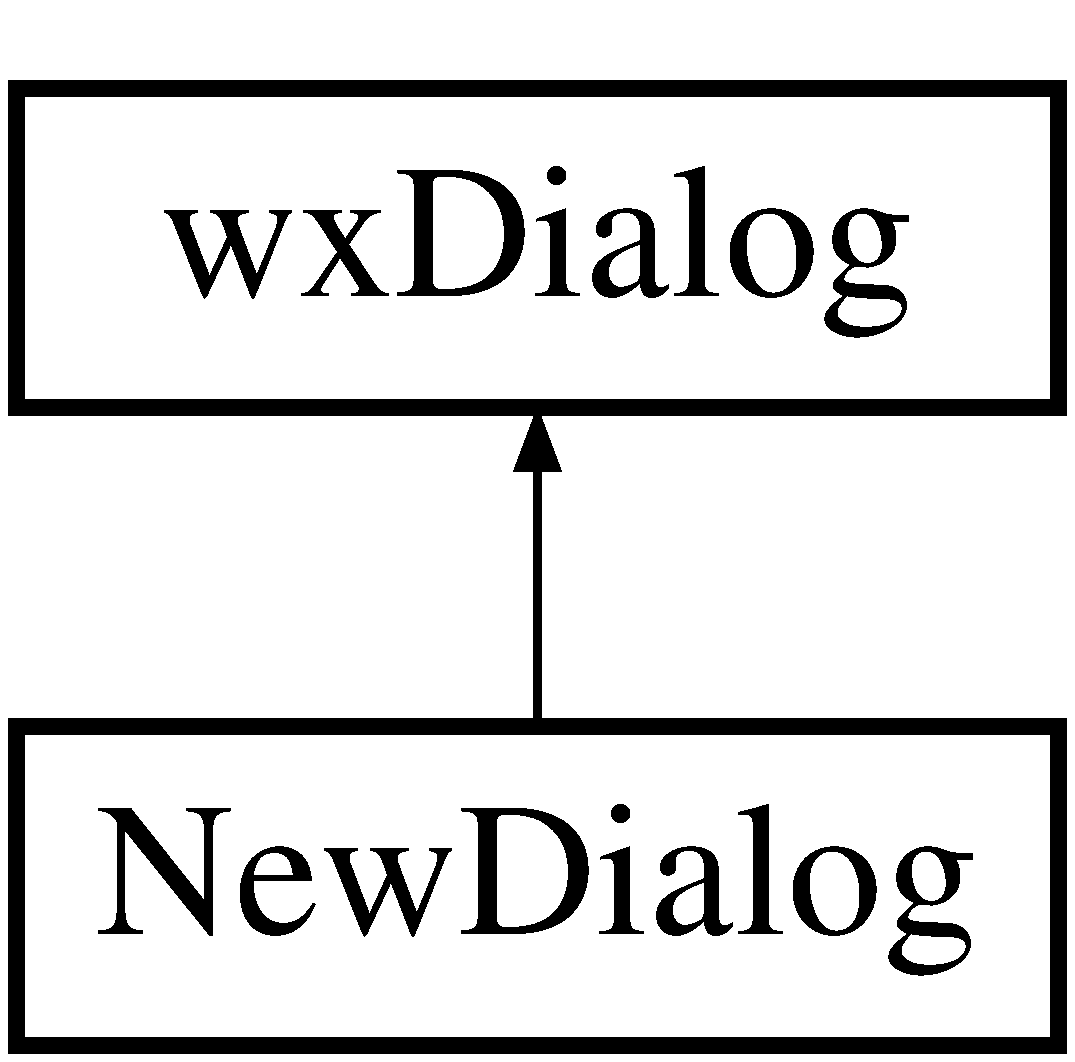
\includegraphics[height=2.000000cm]{class_new_dialog}
\end{center}
\end{figure}
\subsection*{Public Member Functions}
\begin{DoxyCompactItemize}
\item 
\hypertarget{class_new_dialog_a6910ade228aac35f03cb8840d12b79f7}{{\bfseries New\+Dialog} (wx\+Window $\ast$parent, wx\+Window\+I\+D id=wx\+I\+D\+\_\+\+A\+N\+Y)}\label{class_new_dialog_a6910ade228aac35f03cb8840d12b79f7}

\item 
\hypertarget{class_new_dialog_a0ff3a246f99184deffc5d89589725b73}{void {\bfseries Init\+With\+Icon\+Items} (bool with\+Text, bool same\+Icon)}\label{class_new_dialog_a0ff3a246f99184deffc5d89589725b73}

\item 
\hypertarget{class_new_dialog_aaff9ed71f3680ab6017d7189da769e63}{void {\bfseries File\+Selected} (wx\+Command\+Event \&W\+X\+U\+N\+U\+S\+E\+D(event))}\label{class_new_dialog_aaff9ed71f3680ab6017d7189da769e63}

\item 
\hypertarget{class_new_dialog_a235c2e6d2a3b472bfd00c29384e199e3}{void {\bfseries On\+Cancel} (wx\+Command\+Event \&W\+X\+U\+N\+U\+S\+E\+D(event))}\label{class_new_dialog_a235c2e6d2a3b472bfd00c29384e199e3}

\end{DoxyCompactItemize}
\subsection*{Public Attributes}
\begin{DoxyCompactItemize}
\item 
\hypertarget{class_new_dialog_a0229a4f4a97df11a218c470f0e55539f}{wx\+Text\+Ctrl $\ast$ {\bfseries Text\+Ctrl4}}\label{class_new_dialog_a0229a4f4a97df11a218c470f0e55539f}

\item 
\hypertarget{class_new_dialog_a51c03c48fc0c91e7947aa2c8e2582d32}{wx\+List\+Ctrl $\ast$ {\bfseries List\+Ctrl1}}\label{class_new_dialog_a51c03c48fc0c91e7947aa2c8e2582d32}

\item 
\hypertarget{class_new_dialog_a8deabd2e654c2dbb3d32bf175cc161bd}{wx\+Static\+Text $\ast$ {\bfseries Static\+Text2}}\label{class_new_dialog_a8deabd2e654c2dbb3d32bf175cc161bd}

\item 
\hypertarget{class_new_dialog_ae086f43080501f161ee1b3b8a027c114}{wx\+String {\bfseries Test}}\label{class_new_dialog_ae086f43080501f161ee1b3b8a027c114}

\item 
\hypertarget{class_new_dialog_ac67d8f0d8090b9d3eee721907b5f7511}{wx\+Button $\ast$ {\bfseries Button1}}\label{class_new_dialog_ac67d8f0d8090b9d3eee721907b5f7511}

\item 
\hypertarget{class_new_dialog_acf9a3f337785cf4ac5bbff1699187e23}{wx\+Panel $\ast$ {\bfseries Panel1}}\label{class_new_dialog_acf9a3f337785cf4ac5bbff1699187e23}

\item 
\hypertarget{class_new_dialog_a55766963c57d72db947c9cddae1dbf61}{wx\+Static\+Text $\ast$ {\bfseries Static\+Text1}}\label{class_new_dialog_a55766963c57d72db947c9cddae1dbf61}

\item 
\hypertarget{class_new_dialog_ae85d5afd90d11deeb80d89944fcc1a10}{wx\+Static\+Text $\ast$ {\bfseries Static\+Text3}}\label{class_new_dialog_ae85d5afd90d11deeb80d89944fcc1a10}

\item 
\hypertarget{class_new_dialog_a1305415599d313dd00b7aef2a2712ad2}{wx\+Button $\ast$ {\bfseries Button2}}\label{class_new_dialog_a1305415599d313dd00b7aef2a2712ad2}

\item 
\hypertarget{class_new_dialog_a9018c6d38fa57a127b5cae3ce06a5809}{wx\+Panel $\ast$ {\bfseries Panel3}}\label{class_new_dialog_a9018c6d38fa57a127b5cae3ce06a5809}

\item 
\hypertarget{class_new_dialog_a9bc6616941ab92d52566edc34b44ee1e}{wx\+Button $\ast$ {\bfseries Button3}}\label{class_new_dialog_a9bc6616941ab92d52566edc34b44ee1e}

\item 
\hypertarget{class_new_dialog_ad2ef291296f5a3d72af5cd58f28e6ffa}{wx\+Static\+Text $\ast$ {\bfseries Static\+Text5}}\label{class_new_dialog_ad2ef291296f5a3d72af5cd58f28e6ffa}

\item 
\hypertarget{class_new_dialog_aa1b42b667f425ba64b29cc610afcd2ba}{wx\+Text\+Ctrl $\ast$ {\bfseries Text\+Ctrl2}}\label{class_new_dialog_aa1b42b667f425ba64b29cc610afcd2ba}

\item 
\hypertarget{class_new_dialog_a99dbe209b8492d0b0b614c5f7418e47a}{wx\+Tree\+Ctrl $\ast$ {\bfseries Tree\+Ctrl1}}\label{class_new_dialog_a99dbe209b8492d0b0b614c5f7418e47a}

\item 
\hypertarget{class_new_dialog_ac2aed46d40e68eb26bf991d0adb86b9a}{wx\+Text\+Ctrl $\ast$ {\bfseries Text\+Ctrl1}}\label{class_new_dialog_ac2aed46d40e68eb26bf991d0adb86b9a}

\item 
\hypertarget{class_new_dialog_a9ce94be93f78237eba4e75afa0c18d1c}{wx\+Panel $\ast$ {\bfseries Panel2}}\label{class_new_dialog_a9ce94be93f78237eba4e75afa0c18d1c}

\item 
\hypertarget{class_new_dialog_a21f6e52d34b71e48a9666a71c6329be3}{wx\+Text\+Ctrl $\ast$ {\bfseries Text\+Ctrl5}}\label{class_new_dialog_a21f6e52d34b71e48a9666a71c6329be3}

\item 
\hypertarget{class_new_dialog_aa016c49b89b49650e13d3ca9e3ebef5e}{wx\+Static\+Text $\ast$ {\bfseries Static\+Text4}}\label{class_new_dialog_aa016c49b89b49650e13d3ca9e3ebef5e}

\item 
\hypertarget{class_new_dialog_ac01f7008aeb34554abfe2d0ac5b7e5bf}{wx\+Text\+Ctrl $\ast$ {\bfseries Text\+Ctrl3}}\label{class_new_dialog_ac01f7008aeb34554abfe2d0ac5b7e5bf}

\item 
\hypertarget{class_new_dialog_a5d90462e4b115b19dc740f33e802cee2}{wx\+Image\+List $\ast$ {\bfseries m\+\_\+image\+List\+Small}}\label{class_new_dialog_a5d90462e4b115b19dc740f33e802cee2}

\item 
\hypertarget{class_new_dialog_a38ef13059eca81dc88345f5858bc7cad}{bool {\bfseries File\+Select}}\label{class_new_dialog_a38ef13059eca81dc88345f5858bc7cad}

\end{DoxyCompactItemize}
\subsection*{Static Protected Attributes}
\begin{DoxyCompactItemize}
\item 
\hypertarget{class_new_dialog_a20c2ad7818b872789ca2fb21e6806e20}{static const long {\bfseries I\+D\+\_\+\+T\+R\+E\+E\+C\+T\+R\+L1} = wx\+New\+Id()}\label{class_new_dialog_a20c2ad7818b872789ca2fb21e6806e20}

\item 
\hypertarget{class_new_dialog_a0aef7d7ae3bb368a87b0ce504b77ec9c}{static const long {\bfseries I\+D\+\_\+\+L\+I\+S\+T\+C\+T\+R\+L1} = wx\+New\+Id()}\label{class_new_dialog_a0aef7d7ae3bb368a87b0ce504b77ec9c}

\item 
\hypertarget{class_new_dialog_ada2b1a5c697b6f900d2fa7b8e13594cc}{static const long {\bfseries I\+D\+\_\+\+T\+E\+X\+T\+C\+T\+R\+L5} = wx\+New\+Id()}\label{class_new_dialog_ada2b1a5c697b6f900d2fa7b8e13594cc}

\item 
\hypertarget{class_new_dialog_a5bea1bb9a7c5623bcdfcfc0490e1a4b9}{static const long {\bfseries I\+D\+\_\+\+P\+A\+N\+E\+L1} = wx\+New\+Id()}\label{class_new_dialog_a5bea1bb9a7c5623bcdfcfc0490e1a4b9}

\item 
\hypertarget{class_new_dialog_ad48cccd177e5359fcff6daa6c1750485}{static const long {\bfseries I\+D\+\_\+\+T\+E\+X\+T\+C\+T\+R\+L4} = wx\+New\+Id()}\label{class_new_dialog_ad48cccd177e5359fcff6daa6c1750485}

\item 
\hypertarget{class_new_dialog_a873b13e70226c0c50c58a2a31e7c5e6a}{static const long {\bfseries I\+D\+\_\+\+T\+E\+X\+T\+C\+T\+R\+L1} = wx\+New\+Id()}\label{class_new_dialog_a873b13e70226c0c50c58a2a31e7c5e6a}

\item 
\hypertarget{class_new_dialog_ad2715217af15a1602a5cbef0c247862e}{static const long {\bfseries I\+D\+\_\+\+T\+E\+X\+T\+C\+T\+R\+L3} = wx\+New\+Id()}\label{class_new_dialog_ad2715217af15a1602a5cbef0c247862e}

\item 
\hypertarget{class_new_dialog_af636619ae6f8c134f2eafce30a3a9c25}{static const long {\bfseries I\+D\+\_\+\+T\+E\+X\+T\+C\+T\+R\+L2} = wx\+New\+Id()}\label{class_new_dialog_af636619ae6f8c134f2eafce30a3a9c25}

\item 
\hypertarget{class_new_dialog_a19d3f77775795f2dffa1c779f42e26e6}{static const long {\bfseries I\+D\+\_\+\+B\+U\+T\+T\+O\+N1} = wx\+New\+Id()}\label{class_new_dialog_a19d3f77775795f2dffa1c779f42e26e6}

\item 
\hypertarget{class_new_dialog_a7a0d550ea58e2fadee155ac45a46c685}{static const long {\bfseries I\+D\+\_\+\+S\+T\+A\+T\+I\+C\+T\+E\+X\+T1} = wx\+New\+Id()}\label{class_new_dialog_a7a0d550ea58e2fadee155ac45a46c685}

\item 
\hypertarget{class_new_dialog_a3a9f98f40ade560c2c9710b7195c680f}{static const long {\bfseries I\+D\+\_\+\+S\+T\+A\+T\+I\+C\+T\+E\+X\+T2} = wx\+New\+Id()}\label{class_new_dialog_a3a9f98f40ade560c2c9710b7195c680f}

\item 
\hypertarget{class_new_dialog_ac1b9d026a8c92df5e7c7284aaf788a00}{static const long {\bfseries I\+D\+\_\+\+S\+T\+A\+T\+I\+C\+T\+E\+X\+T3} = wx\+New\+Id()}\label{class_new_dialog_ac1b9d026a8c92df5e7c7284aaf788a00}

\item 
\hypertarget{class_new_dialog_a55ba13f3328ccadcf9a171d30558b06f}{static const long {\bfseries I\+D\+\_\+\+S\+T\+A\+T\+I\+C\+T\+E\+X\+T4} = wx\+New\+Id()}\label{class_new_dialog_a55ba13f3328ccadcf9a171d30558b06f}

\item 
\hypertarget{class_new_dialog_a0be6b5ca68521b8a6378d3d74d6e7690}{static const long {\bfseries I\+D\+\_\+\+P\+A\+N\+E\+L2} = wx\+New\+Id()}\label{class_new_dialog_a0be6b5ca68521b8a6378d3d74d6e7690}

\item 
\hypertarget{class_new_dialog_a6c4dea442453e0a5a160f9c27a755d0d}{static const long {\bfseries I\+D\+\_\+\+S\+T\+A\+T\+I\+C\+T\+E\+X\+T5} = wx\+New\+Id()}\label{class_new_dialog_a6c4dea442453e0a5a160f9c27a755d0d}

\item 
\hypertarget{class_new_dialog_a0784f1e99fc71920ff777b3db5a1c5e7}{static const long {\bfseries I\+D\+\_\+\+P\+A\+N\+E\+L3} = wx\+New\+Id()}\label{class_new_dialog_a0784f1e99fc71920ff777b3db5a1c5e7}

\end{DoxyCompactItemize}


The documentation for this class was generated from the following files\+:\begin{DoxyCompactItemize}
\item 
New\+Dialog.\+h\item 
New\+Dialog.\+cpp\end{DoxyCompactItemize}

\hypertarget{class_new_file}{\section{New\+File Class Reference}
\label{class_new_file}\index{New\+File@{New\+File}}
}
Inheritance diagram for New\+File\+:\begin{figure}[H]
\begin{center}
\leavevmode
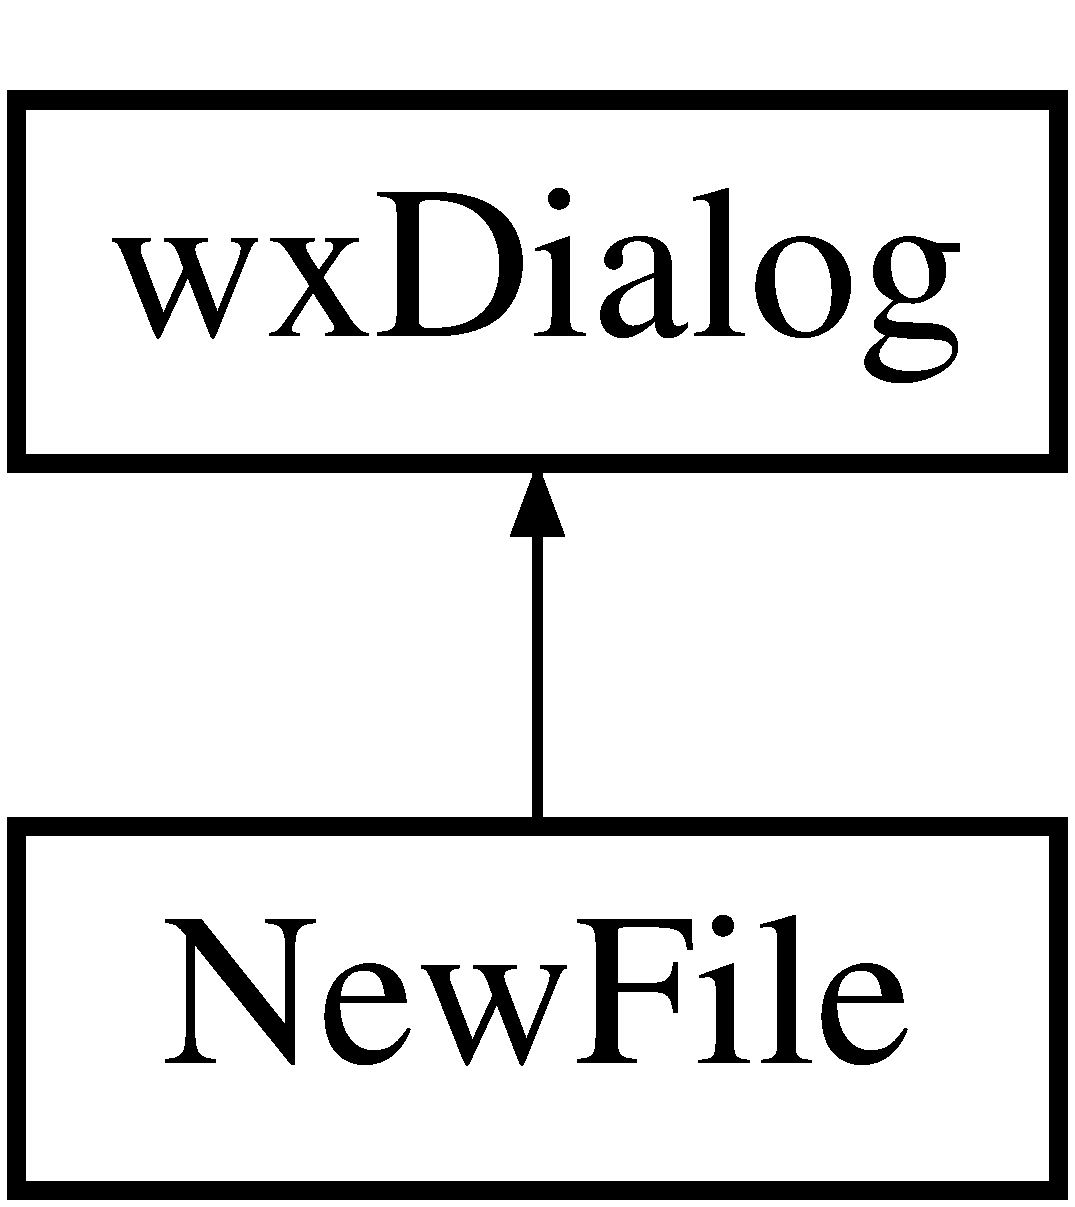
\includegraphics[height=2.000000cm]{class_new_file}
\end{center}
\end{figure}
\subsection*{Public Member Functions}
\begin{DoxyCompactItemize}
\item 
\hypertarget{class_new_file_a3c3de6b98a37f5a2a8123d1ade4d7dbc}{{\bfseries New\+File} (wx\+Window $\ast$parent, wx\+Window\+I\+D id=wx\+I\+D\+\_\+\+A\+N\+Y)}\label{class_new_file_a3c3de6b98a37f5a2a8123d1ade4d7dbc}

\end{DoxyCompactItemize}
\subsection*{Public Attributes}
\begin{DoxyCompactItemize}
\item 
\hypertarget{class_new_file_aabc5d2a67ee13b42367e29dc3e86a24b}{wx\+Text\+Ctrl $\ast$ {\bfseries Text\+Ctrl4}}\label{class_new_file_aabc5d2a67ee13b42367e29dc3e86a24b}

\item 
\hypertarget{class_new_file_a0ab18a21aaa7b8461187298103c88b15}{wx\+Static\+Text $\ast$ {\bfseries Static\+Text2}}\label{class_new_file_a0ab18a21aaa7b8461187298103c88b15}

\item 
\hypertarget{class_new_file_a8aca33e291653b42e165f9ed714e570b}{wx\+Button $\ast$ {\bfseries Button1}}\label{class_new_file_a8aca33e291653b42e165f9ed714e570b}

\item 
\hypertarget{class_new_file_ac373a3497dba10fb7fdd4791d035a45e}{wx\+Panel $\ast$ {\bfseries Panel1}}\label{class_new_file_ac373a3497dba10fb7fdd4791d035a45e}

\item 
\hypertarget{class_new_file_a53f78576920e0cdda246b39be2971ba0}{wx\+Static\+Text $\ast$ {\bfseries Static\+Text1}}\label{class_new_file_a53f78576920e0cdda246b39be2971ba0}

\item 
\hypertarget{class_new_file_a390c9933e2372c3d6d6ac8d5d118a133}{wx\+Static\+Text $\ast$ {\bfseries Static\+Text3}}\label{class_new_file_a390c9933e2372c3d6d6ac8d5d118a133}

\item 
\hypertarget{class_new_file_adb37e127a0aadfc1959da1e553bf8ba3}{wx\+Button $\ast$ {\bfseries Button2}}\label{class_new_file_adb37e127a0aadfc1959da1e553bf8ba3}

\item 
\hypertarget{class_new_file_ac2ba018625f89e584d251d396eab85c8}{wx\+Panel $\ast$ {\bfseries Panel3}}\label{class_new_file_ac2ba018625f89e584d251d396eab85c8}

\item 
\hypertarget{class_new_file_a589d8e9a6d151f2495567fb07ac59744}{wx\+Button $\ast$ {\bfseries Button3}}\label{class_new_file_a589d8e9a6d151f2495567fb07ac59744}

\item 
\hypertarget{class_new_file_ac5187ae498298e75e13a40febffcfd4c}{wx\+Static\+Text $\ast$ {\bfseries Static\+Text5}}\label{class_new_file_ac5187ae498298e75e13a40febffcfd4c}

\item 
\hypertarget{class_new_file_ad8f1cd05cc0b52d95d11ffa002707269}{wx\+Text\+Ctrl $\ast$ {\bfseries Text\+Ctrl2}}\label{class_new_file_ad8f1cd05cc0b52d95d11ffa002707269}

\item 
\hypertarget{class_new_file_af7e4308f62d6a1e9167361f684ad870c}{wx\+Text\+Ctrl $\ast$ {\bfseries Text\+Ctrl1}}\label{class_new_file_af7e4308f62d6a1e9167361f684ad870c}

\item 
\hypertarget{class_new_file_abab5c0fd3691dabbad483ede1068b0c4}{wx\+Panel $\ast$ {\bfseries Panel2}}\label{class_new_file_abab5c0fd3691dabbad483ede1068b0c4}

\item 
\hypertarget{class_new_file_aeb461af09d816293a60876bbfabe2166}{wx\+Static\+Text $\ast$ {\bfseries Static\+Text4}}\label{class_new_file_aeb461af09d816293a60876bbfabe2166}

\item 
\hypertarget{class_new_file_a38e571ff53e73252976fbb7b55d4d55e}{wx\+Text\+Ctrl $\ast$ {\bfseries Text\+Ctrl3}}\label{class_new_file_a38e571ff53e73252976fbb7b55d4d55e}

\end{DoxyCompactItemize}
\subsection*{Static Protected Attributes}
\begin{DoxyCompactItemize}
\item 
\hypertarget{class_new_file_a11038cae655dfcb441991ffad187114e}{static const long {\bfseries I\+D\+\_\+\+P\+A\+N\+E\+L1} = wx\+New\+Id()}\label{class_new_file_a11038cae655dfcb441991ffad187114e}

\item 
\hypertarget{class_new_file_a3464cf15024fb9e49571d24d9b2d0d40}{static const long {\bfseries I\+D\+\_\+\+T\+E\+X\+T\+C\+T\+R\+L4} = wx\+New\+Id()}\label{class_new_file_a3464cf15024fb9e49571d24d9b2d0d40}

\item 
\hypertarget{class_new_file_a1125c518d89dbec295e46240a53bf016}{static const long {\bfseries I\+D\+\_\+\+T\+E\+X\+T\+C\+T\+R\+L1} = wx\+New\+Id()}\label{class_new_file_a1125c518d89dbec295e46240a53bf016}

\item 
\hypertarget{class_new_file_aeee3c478ec5cca687c3c111db5f5b0ff}{static const long {\bfseries I\+D\+\_\+\+T\+E\+X\+T\+C\+T\+R\+L3} = wx\+New\+Id()}\label{class_new_file_aeee3c478ec5cca687c3c111db5f5b0ff}

\item 
\hypertarget{class_new_file_a43a3a036cfb63e625ce85b8d70e0b0ab}{static const long {\bfseries I\+D\+\_\+\+T\+E\+X\+T\+C\+T\+R\+L2} = wx\+New\+Id()}\label{class_new_file_a43a3a036cfb63e625ce85b8d70e0b0ab}

\item 
\hypertarget{class_new_file_a49617943e524eb0a5fa7e156c19f2b29}{static const long {\bfseries I\+D\+\_\+\+B\+U\+T\+T\+O\+N1} = wx\+New\+Id()}\label{class_new_file_a49617943e524eb0a5fa7e156c19f2b29}

\item 
\hypertarget{class_new_file_a680b314362e4c8d2f76a51e66c9b3b27}{static const long {\bfseries I\+D\+\_\+\+S\+T\+A\+T\+I\+C\+T\+E\+X\+T1} = wx\+New\+Id()}\label{class_new_file_a680b314362e4c8d2f76a51e66c9b3b27}

\item 
\hypertarget{class_new_file_a76f89e881f24da2e1789df6626b1e081}{static const long {\bfseries I\+D\+\_\+\+S\+T\+A\+T\+I\+C\+T\+E\+X\+T2} = wx\+New\+Id()}\label{class_new_file_a76f89e881f24da2e1789df6626b1e081}

\item 
\hypertarget{class_new_file_a41404774e082603f292e133b7e7d4449}{static const long {\bfseries I\+D\+\_\+\+S\+T\+A\+T\+I\+C\+T\+E\+X\+T3} = wx\+New\+Id()}\label{class_new_file_a41404774e082603f292e133b7e7d4449}

\item 
\hypertarget{class_new_file_a709e0c5c241bb616a7b8a72f65cbe783}{static const long {\bfseries I\+D\+\_\+\+S\+T\+A\+T\+I\+C\+T\+E\+X\+T4} = wx\+New\+Id()}\label{class_new_file_a709e0c5c241bb616a7b8a72f65cbe783}

\item 
\hypertarget{class_new_file_aebe71a5c2402db2b186b4470bfb11017}{static const long {\bfseries I\+D\+\_\+\+P\+A\+N\+E\+L2} = wx\+New\+Id()}\label{class_new_file_aebe71a5c2402db2b186b4470bfb11017}

\item 
\hypertarget{class_new_file_afe43b64bf0068a3fa5bfb080671ec22e}{static const long {\bfseries I\+D\+\_\+\+S\+T\+A\+T\+I\+C\+T\+E\+X\+T5} = wx\+New\+Id()}\label{class_new_file_afe43b64bf0068a3fa5bfb080671ec22e}

\item 
\hypertarget{class_new_file_a200e4e0dd348ae126befc311f3228388}{static const long {\bfseries I\+D\+\_\+\+P\+A\+N\+E\+L3} = wx\+New\+Id()}\label{class_new_file_a200e4e0dd348ae126befc311f3228388}

\end{DoxyCompactItemize}


The documentation for this class was generated from the following files\+:\begin{DoxyCompactItemize}
\item 
New\+File.\+h\item 
New\+File.\+cpp\end{DoxyCompactItemize}

\hypertarget{struct_style_info}{\section{Style\+Info Struct Reference}
\label{struct_style_info}\index{Style\+Info@{Style\+Info}}
}
\subsection*{Public Attributes}
\begin{DoxyCompactItemize}
\item 
\hypertarget{struct_style_info_a85cd3b65b5d8dda7c0ad9b0ab43c4850}{const wx\+Char $\ast$ {\bfseries name}}\label{struct_style_info_a85cd3b65b5d8dda7c0ad9b0ab43c4850}

\item 
\hypertarget{struct_style_info_ac012a82887301cbcbc08e2bdd660eb3c}{const wx\+Char $\ast$ {\bfseries foreground}}\label{struct_style_info_ac012a82887301cbcbc08e2bdd660eb3c}

\item 
\hypertarget{struct_style_info_aee79fdf6f6958597d36c453ab4bcddc8}{const wx\+Char $\ast$ {\bfseries background}}\label{struct_style_info_aee79fdf6f6958597d36c453ab4bcddc8}

\item 
\hypertarget{struct_style_info_af042851ce2370836f61abd1c3850b6f2}{const wx\+Char $\ast$ {\bfseries fontname}}\label{struct_style_info_af042851ce2370836f61abd1c3850b6f2}

\item 
\hypertarget{struct_style_info_a48d89f89cde92d8ffb7d5eb5021ee48c}{int {\bfseries fontsize}}\label{struct_style_info_a48d89f89cde92d8ffb7d5eb5021ee48c}

\item 
\hypertarget{struct_style_info_a3b8deeae812039660a177e98e749d735}{int {\bfseries fontstyle}}\label{struct_style_info_a3b8deeae812039660a177e98e749d735}

\item 
\hypertarget{struct_style_info_a50a9aa929cce38347977e33a5970b046}{int {\bfseries lettercase}}\label{struct_style_info_a50a9aa929cce38347977e33a5970b046}

\end{DoxyCompactItemize}


The documentation for this struct was generated from the following file\+:\begin{DoxyCompactItemize}
\item 
prefs.\+h\end{DoxyCompactItemize}

%--- End generated contents ---

% Index
\newpage
\phantomsection
\addcontentsline{toc}{chapter}{Index}
\printindex

\end{document}
